

\documentclass{article}
\author {Yuke Chen, Yixiang Gong, Tiffani Rachman, Kensuke Tamura, Tudor Vasile, Tudor Zugravu}
\title{Kings College London \\ Group Project  (7CCSMGPR).  \\ Final Report} 
\usepackage{a4wide}
\usepackage{graphicx}
\usepackage{float}
\usepackage{multirow}
\usepackage{color}
\usepackage{array}
\newcolumntype{L}{>{\centering\arraybackslash}m{3cm}}
\usepackage{tabularx}
\usepackage{subcaption}
\usepackage{listings}

\begin{document}
	\renewcommand*\contentsname{Contents}
	\maketitle
	\pagenumbering{arabic}
	\tableofcontents

	\paragraph{}
	\fontsize{12}{12}\selectfont

\newpage
\section{Introduction}

	
	Team kchat has been assigned to create a multi-platform, multi-user chat application. In the early stages of the project, the various problems that could be faced in terms of end user clients and communication between them have been discovered. Some identified problems ordered by priority are: How will the communication channel work? What are the end user devices that are going to be used? What are the purposes of both the client and the server and what are their functions?\par
	The questions asked above lead to the establishment of the system's aims, which were made clearer when research was performed. These problems have been solved with the use of a server and a communication framework.\par
	During this process0 various coding, team-management and problem solving issues have been encountered, which have been resolved and are mentioned throughout this report. These issues could only have been solved with the use of our adapted agile software methodology, which has helped the team to develop stronger management, communication and time-management skills by responding to changes early on in the process and helping one another if issues occurred. At the end of the process the requirements were completer, the team having gained new understanding of the system's functional complexity, communicating effectively as a team when encountering new problems and building strong confidence and teamwork. 
	
	\section{Review}
	
	\textbf{\underline{Related Work}}
	
	\begin{enumerate}
		\item MSN messenger
	
		\begin{figure}[h]
		\centering
		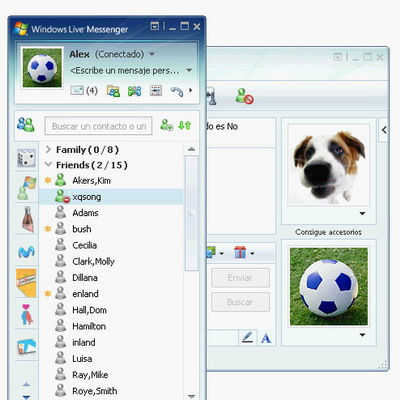
\includegraphics[scale=0.4]{msn-messenger-3.jpg}
		\cite{msnimage}
		\caption{Example MSN's client side UI}
		\end{figure}
		
	\textit{Msn is an instant messenger created by Microsoft so you can communicate with all your friends from all around the world, you can instantly chat or webcam as well as type, or have a video chat if you own a webcam and mircophone.\\ \\MSN is the fancy way of getting hold of your mates when there online and offline as you can change your font, name and status to offline, online, busy, out to lunch and away.}\par \cite{msndesc}

	When evaluating MSN messenger, we discovered features which, at the time, were considered to be of an exceptional standard. One advantage of MSN messenger is that has the ability to communicate with anyone around the world provided that both participants have a reliable Internet connection. New features were gradually added such as web-cam support, file sending features and the ability to create chat rooms quick and easy. Over time, MSN messenger has evolved in today's modern businesses as Lync. Corporations made use of Lync features such as video conferencing, meeting planner and business style calendar. \par
	
	Some difficulties were also outlined from MSN's functionalities, such as the constant drop of connection, meaning that some of the users' Internet speeds did not match MSN's required performance. Other identified problems are the occurance of online cyber bullying and the sending of spam messages many times to multiple users. These were some issues that needed to be addressed in our applications.\par 
	
		\item Facebook messenger
	
	\begin{figure}[h]
		\centering
		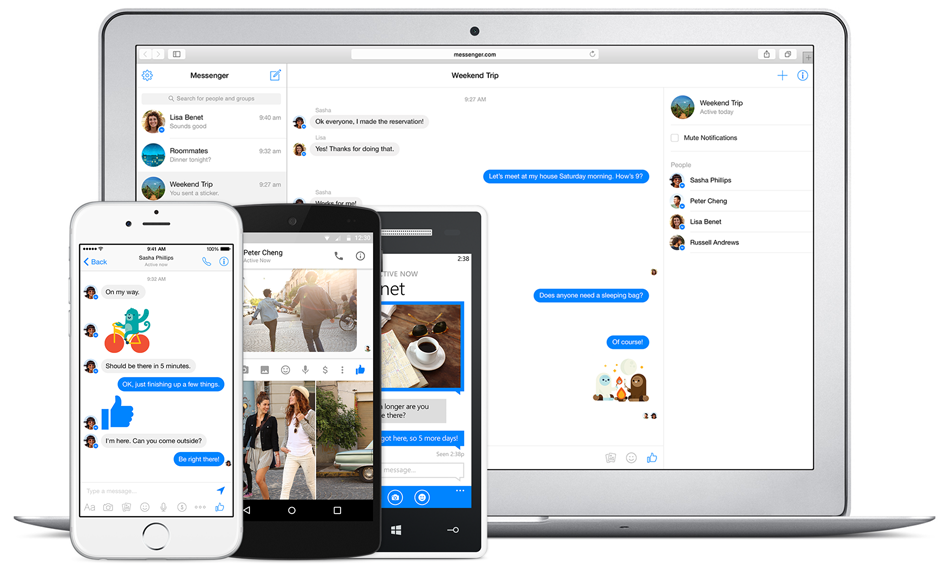
\includegraphics[scale=0.3]{facebookUI.png}
		\cite{facebookmessenger}
		\caption{Facebook's user interfaces on multiple platforms}
	\end{figure}

		\textit{Facebook may be accessed by a large range of desktops, laptops, tablet computers, and smartphones over the Internet and mobile networks. After registering to use the site, users can create a user profile indicating their name, occupation, schools attended and so on. Users can add other users as "friends", exchange messages, post status updates and digital photos, share digital videos and links, use various software applications ("apps"), and receive notifications when others update their profiles or make posts. Additionally, users may join common-interest user groups organized by workplace, school, hobbies or other topics, and categorize their friends into lists such as "People From Work" or "Close Friends". In groups, editors can pin posts to top. Additionally, users can complain about or block unpleasant people. Because of the large volume of data that users submit to the service.}\par \cite{facebookdesc}
	
	\newpage
	Facebook's messenger provides extremely fast message transmission, the recorded speeds beoing faster than sending a message on the mobile browser. Users can make calls, send pictures, links, videos, stickers and many other types of media. Facebook messenger also provides calls via Wi-fi or 3G network and, more importantly, allows the use of sending messages off-line.  \par
	
	Identified disadvantages include the usage of device space upon installation, taking over 100MB. For such a simple application the space grows depending on the amount of add-ons that are downloaded for the application. Another issue we have found is the drainage of battery life.\cite{facebookbattery}. Facebook uses many audio multimedia threads which are running in the phone's background. It has addressed this issue and will continue to apply fixes and hopefully solve this problem in the future. \par
	
	\item Apple Imessage
	\end{enumerate}
	
		\begin{figure}[h]
		\centering
		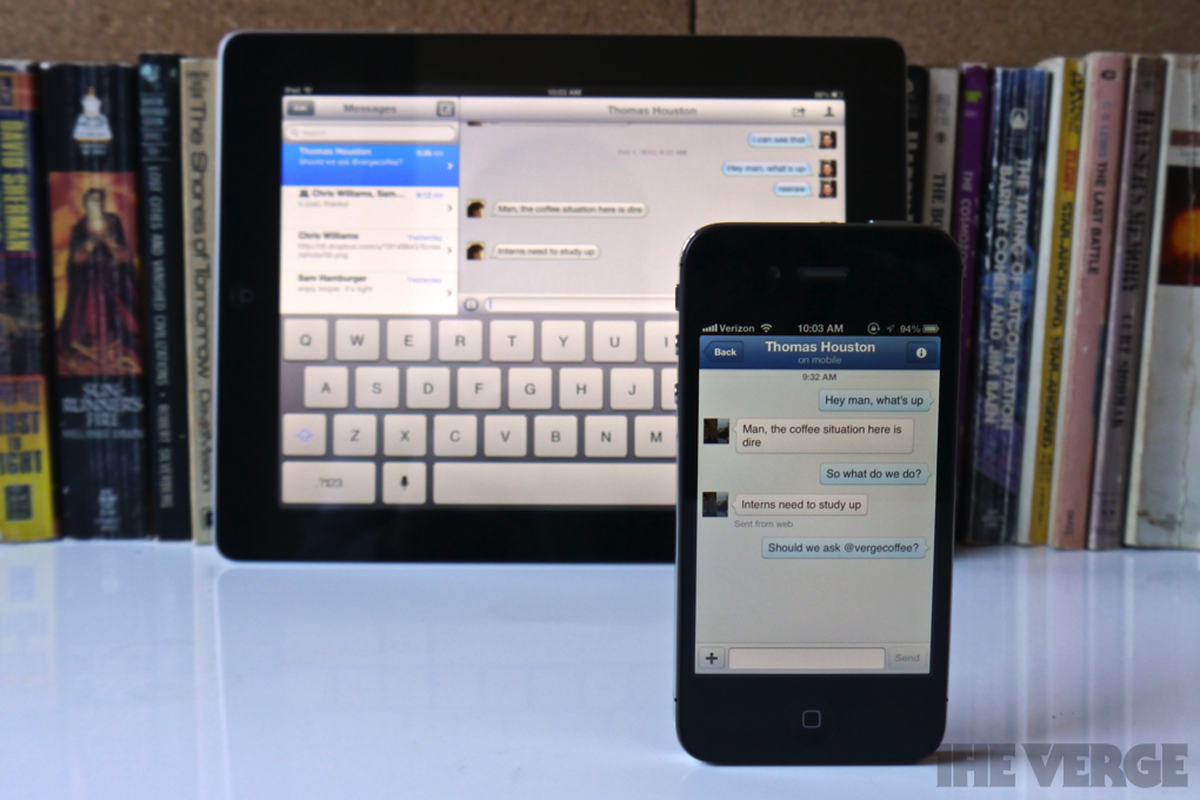
\includegraphics[scale=0.3]{facebook_messenger.png}
		\cite{imessagephoto}
		\caption{Facebook's user interfaces on multiple platforms}
	\end{figure}

	\textit{iMessage allows users to send texts, documents, photos, videos, contact information, and group messages over Wi-Fi, mobile phone Internet access, or other forms of Internet access to other iOS or macOS users, thus providing an alternative to standard SMS/MMS messaging for most users with devices running iOS 5 or later.}\\

	\textit{iMessage is accessible through the Messages app on an iPhone, iPad or iPod touch running iOS 5 or later or on a Mac running OS X Mountain Lion or later. Owners of these devices can register one or more email addresses with Apple, and, additionally, iPhone owners can register their phone numbers with Apple, provided their carrier is supported. When a message is sent to a mobile number, Messages will check with Apple if the mobile number is set up for iMessage. If it is not, the message will seamlessly transition from iMessage to SMS.}\par \cite{imessagedesc}
	
	Some advantages of iMessage include rapid, unlimited transmission of messages with good signal even in more difficult areas and the ability of transferring accounts. iMessage contains an elegant user interface which is easy to operate. However, some limitations include a waste of data plan if used constantly and without care, the fact that it could not be deleted from iOS phones and that it is not available to Android users. \\
	
	Based on the team-performed research, we reflected to move onto the next step and to form our requirements based on the positive identified features, keeping in mind to also address and hopefully solve the negative aspects of existing software.
	
	\section{Requirements}
	
	The scope of this project is to develop a multi-platform application designed to allow multi-user communication.\\
	During the early stages, a list of different features the application should contain have been planned out, these derived by analyzing the user's point of view and the research performed. These are displayed as platform and functional requirements.\par
	
	\subsection{Platform Requirements}
	\begin{itemize}
		\item P1 - Design a responsive login page, connect to the server and then check the user's input.
		\item P2 - Design a registration page, send the user's credentials to the server and check with existing stored data. In case of conflicts, reply to the user.
		\item P3 - Design the home page/menu that is responsible for displaying the correct chats, groups and data upon successful login.
		\item P4 - Design windows or menus that are responsible for holding contact information such as sent and received requests, as well as contacts themselves.
		\item P5 - Design a chat window which should display the messages clearly, along with the user's profile and the last message timestamp.
		\item P6 - Design the user's profile page and allow him/her to change any details, including the profile image.
		\item P7 - Allow the user to create a group, add members from his contacts page and delete the group in case of ownership. Otherwise, the user should be able to leave the group.
		\item P8 - Allow the user to delete his own account and provide a challenge, if possible, for the user before confirming.
		\item P9 - Allow the user to delete and accept contacts before starting a conversation.
	\end{itemize}

\subsection{Functional Requirements}
\begin{itemize}
	\item FR1 - Set up a cloud server that is responsible for managing the user accounts' data and message transmission functionalities.
	\item FR2 - The server should run by itself constantly and under a heavy load.
	\item FR3 - The client should perform REST requests for high load information and use a different means of communication for transmitting messages.
	\item FR4 - The server should separate receiving messages and receiving other types of information by string, inserting the data in the correct relational database table.
	\item FR5 - The server should always provide a response to any requests, these messages having to reach the client.
	\item FR6 - The client should still be able to use the application even if there is no Internet available.
	\item FR7 - The client should be able to send messages offline.
	\item FR8 - The client should still be allowed to maintain the session if the mobile application has been sent to the background.
	\item FR9 - Messages should be able to be stored on the client's device for offline browsing.
	\end{itemize}

\subsection{Security Requirements}
\begin{itemize}
	\item S1 - The client should not be allowed to sign in twice with the same account.
	\item S2 - If the session has been destroyed, the client should be directed to the log in.
	\item S3 - The client's password should be hashed and then stored in the database. 
	\item S4 - Messages should be encrypted on transmission and stored locally on the phone in an encrypted format.
	\item S5 - The client's offline databases should clear upon session loss and on logout.\\

	The above requirements describe realistic approaches of all the available features from research and general idea brainstorming. The next phase is to prioritize some of the gathered requirements from the above Table 1 and form concrete specifications. In the case of this project, given the time, equipment and resources, the requirements needed to be broken down and given a priority in the order of highest importance first. 
	
\end{itemize}
\newcolumntype{C}{>{\centering\arraybackslash}X} % centered version of 'X' columns
\begin{table}[H]
	\centering
\begin{tabularx}{17cm}{|c|C|c|}
	\hline
	\textbf{Code} & \textbf{Specification} & \textbf{Priority Importance} \\ \hline
	\hline
		P1&Use the appropriate design components which hide the user input for  the password&High      \\ \hline
	P2&The user interface should have a simple design and views should be re-used for different components. &High          \\ \hline
	P3&Use languages appropriate components as to allow the user interface to be redesigned in order to show the appropriate data  & High     \\ \hline
	P4&Provide responsive text search, which is responsible for querying the specified data appropriately &High      \\ \hline
	P5&Display sent messages on the right side of the screen and display the other users' ones on the other side. They should be identified by a name or icon. Messages should be ordered by timestamp  & High      \\ \hline
	P6&The profile page must contain information about the user, such as email, phone number, biography and username. The profile should contain an image icon which would be helpful for conversation identification.  & High      \\ \hline
	P7& Include in each client a standard of notification: if a group has been deleted, then users must leave the conversation view and be returned to the chat menu. Also, the user interface should be updated to show the list with the group removed.   &  Medium      \\ \hline
	P8& The user should provide his password appropriately and it should be validated by the server. This would eliminate accounts to be deleted by someone else if the user is still in session. & High        \\ \hline
	P9&Contacts should be accepted or deleted. This would also remove the relationship of users and the message conversations should be cleared.     & Medium    \\ \hline
	\hline
	FR1&The cloud server must be constantly available and at a reasonable price. Communication with the server must be easy to set up. &Very High     \\ \hline
	FR2&Choosing a correct cloud server company is essential for management. Some companies provide excellent support services with extended tools used to monitor activity and collect logs.   &Very High    \\ \hline 
	FR3&As REST requests are expensive, one solution would be to group the messages together and send them as a batch. However, this would cause problems since some requests could be lost in transit. One solution would be to use a reliable communication channel which must be bi-directional and responsive.    &  Very High   \\ \hline
	FR4& Received messages should comply to a standard recognizable to multiple devices. Devices must individually manage the data retrieved. Received data must be de-structured, validated and finaly managed on the server side. One example is the use of the JSON format to represent objects. & High   \\ \hline
	FR5& Responses should be alerts for errors where the application must have a interface for listening to the server. Technical errors should not be shown to the client but handled by the system & Medium    \\ \hline
	FR6& The application's availability should not relate to the area's internet bandwidth allocation. The client's application should provide feedback to the by showing a message if there is no internet, before trying to contact the server.  &Medium     \\ \hline
	FR7& If the user's application does go offline, checks should be made ensuring that messages are stored in a buffer and then sent to the correct contact upon re-connection. Messages could be stored in a SQLite database, saved preferences or a persistent data storage and flushed after some time. &  Medium   \\ \hline

\end{tabularx}
\end{table}

\begin{table}[H]
	\centering
	\begin{tabularx}{17cm}{|c|C|c|}
		\hline
		\textbf{Code} & \textbf{Specification} & \textbf{Priority Importance} \\ \hline
		\hline
 
		FR8& The client should not log-in each time the application starts. However, for security reasons, sessions should be kept short.  & Medium    \\ \hline
		FR9& Messages must be stored persistently if the client has an internet connection and must be retrieved depending on the condition of  connection.  & Low     \\ \hline
		\hline
		S1& The client's session must be validated by the server. Another useful check is to validate the device the client uses to sign-in with and to force log out of old sessions. &  Low   \\ \hline
		S2& Each platform must keep track of the duration of client sessions in the form of either cookies or preferences. It would be ideal to remove the client from a session if the Internet connection has been lost. & Medium     \\ \hline
		S3& Hashing algorithms such as MD5 or SHA-256 could be used. For extra protection, the use of salts would make the passwords more difficult to crack, in the case that the server's database has been compromised  & High     \\ \hline
		S4& Messages should be encrypted in the same format as code S3  & Medium    \\ \hline
		S5& Databases should be emptied upon log-out so no unauthorized users could obtain a copy and decode the contents  & Medium    \\ \hline
	\end{tabularx}
\end{table}

	Based on the formalized requirements, it has been decided to form sub teams based on each team member's skill set. These skills included experience in web, Android and iOS only. This was decided to maximize efficiency and provided vital for completing the requirements. The meeting finished with everyone being paired up, forming 3 sub teams. In order to distinguish these teams, the name of the language technology was used for the team name.\par
	
\newpage
	\section{Design}
	\subsection{Workflow}
	
	The workflow of the chat system is based upon the platform and functional requirements, with the target of providing a better user experience. Thus, the functionalities the system offers aim to cover most of the features that users look for in such products.\par
	
	As the clients are meant to be used by one user at a time, login and signup functionalities are provided. When a user logs in, the credentials are sent to the server and verified with the database. The clients feature sessions, allowing the current user to stay logged in. This is possible through validation of the stored credentials at launch. If successful, the private chat window is presented. The system does not allow double login. Whether the used client is one of the mobile application or the web interface, it listens for and acts upon different events sent by the server. One of such events is the disconnect signal sent by the server to any active instances of a user's session upon the successful authentification on a new client.\par
	
	Accessing the private chats window triggers a request to the server, providing a list of all the user's previous conversations, sorted by the last message sent. By selecting one of these, the last 20 messages of that chat will be retrieved from the server. In order to view more messages, the user must scroll to the top of the conversation, triggering the retrieval of 20 more messages.In addition, when a message is sent, the server sends a notification to the other contact. If he/she is in the current chat's window, the new message will appear at the bottom. If not, a notification sound will be played and the conversation will appear at the top of the list automatically.\par
	
	Group chats follow the same pattern of communication. However, the current user has the option of creating a new group, selecting up to 6 contacts and a group image. This triggers the dispach of notifications to the added users, their group chats window showing the new group automatically. In addition, the users can leave groups that they do not own and add members to or delete the groups that they manage. A group deletion will trigger the disappearance of that group from the other members' lists.\par
	
	The clients also provide means of managing the contacts list, with the possibility of sending contact requests, accepting incoming requests and deleting outgoing ones. Upon each of these events, the target contact will receive a notification from the server and their contacts lists will be updated automatically. Moreover, when deleting a contact, the conversation with that particular user will disappear. Selecting a contact list item will provide two options: starting a conversation with that contact, or viewing 	their profile pages. This is done by single tap and long tap respectively, on the mobile clients. Moreover, each user has the option to update their profile details, as well as taking and uploading a new profile picture.\par
	
	As the web platform works on web browsers, it will not be available with no internet connection. However, the mobile applications provide the means of viewing the latest conversations, as well as the possibility of sending messages in an offline mode. This is done by saving the outgoing messages in a buffer, which is sent towards the server upon reconnection to the internet.\par
	\newpage
	\subsection{System Architecture}
	
	The system is based upon a 3-tier architecture, the components being divided in three logical modules: presentation,logic and data. This approach best suits this project due to it's client-server design. Thus, the user interface, the process logic and the data storage and accessibility are implemented individually, providing modularity and easier scallability.\par
	
	The Presentation tier is represented by the user interface and it's purpose is to provide a platform through which information can be visualised, manipulated and entered. It communicates with the other components and outputs the results on the graphical interface provided by the system through the use of visual components such as windows, forms and web pages. The system's Presentation level is composed of the web interface and the iOS and Android mobile applications.\par
	
	\begin{figure}[H]
		\centering
		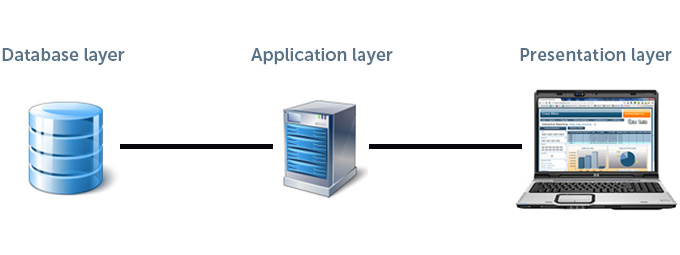
\includegraphics[scale=0.3]{client-server.jpg}
		\caption{3-Tier Architecture}
		\cite{3tierarchitecture}
	\end{figure}

	The users of the chat system view specific information such as their contact list, recent private and group conversations and profile details. In addition, they have access to data manipulation features such as modifying their profile and the groups they are members of. The user interface also provides the means of message input and profile picture upload.\par
	
	The system's functionality conditioning is maintained in the Application tier through the execution of specific processes and handling of the persistent data, allowing control of updates and modifications to the user relevant and system information. Separating the chat system's process logic into an individual layer allows transparent process execution and provides the means of communication between the user interfaces and the database. The Application tier is represented by the server, which is the target of all the client requests. It is responsible with the database queries, data traffic and flow control. However, the main functionality of the server is to securely connect the users and provide the means of communication between them. In order to achieve this, as well as to provide a better user experience for the users, their sessions are managed on the server.
	
	The Data tier is where the data is persistently stored and it includes data manipulation mechanisms, providing an API for the Application layer for access to information. All of the chat system's clients provide interfaces that display the data stored in this layer and all of the input provided by them is centralised here. The system's database structure separates the data based upon user information, relationship between users, messages etc. in order to provide faster access.
	
	Each team was involved in performing their own different model. These models aid our understanding of the system which solves a particular problem. One example is a state machine diagram which outlines the types of states available in a system and the transitions in form of functions that are used to traverse from one state to another. This has helped the team to plan the problem of UI views an application should have and which functions change the views. \par
	 
	\newpage
	\subsection{\underline{\textbf{Android}}}
	One of the diagrams constructed by team android is an activity state machine diagram. Each state represents the views available that possibly a client could visit. Each state is unique since it reveals its operations that a client could trigger. Triggering the correct functions would direct the client to a new state represented as a new view.
	
	\begin{figure}[H]
		\centering
		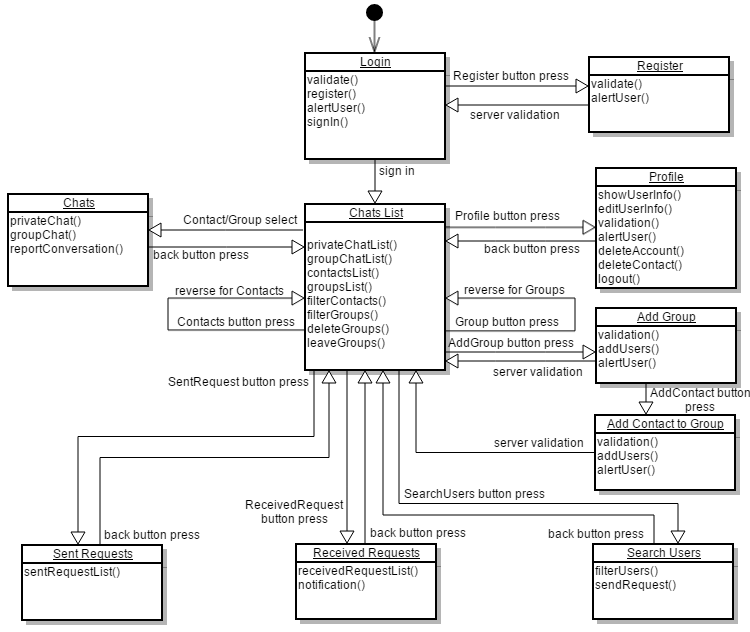
\includegraphics[scale=0.7]{androidActivity.png}
		\caption{Android State Machine Activity Diagram}
	\end{figure}

	The advantage of using a state machine consists of simplicity in terms of transitions. The client would start at the black dot and then transition from state to state, in our case which would be endlessly until the application has been killed off. This diagram is more simple to visualize than a class diagram since it contains only the most needed functions which are necessary to a client. One disadvantage is maintainability since if new states are added the complexity of transitions would also increase.
	
	\newpage
	\subsection{\underline{\textbf{iOS}}}
	One of the three clients of the chat system is an iOS application, targeting one of the most used mobile operating systems today. For this reason, the implementation of the iOS application follows a structure containing specific elements, best practices that provide well-established module organisation throughout the project, as well as design patterns. One such design pattern is the Model-View-Controller, which defines the objects used in the system as one of three roles: Model, View or Controller. This not only establishes their scope, but also the way they communicate. Most of these objects are reusable throughout the application, providing a more seamless way of extending the app.
	
	\begin{figure}[H]
		
		\begin{subfigure}{\linewidth}
			\centering
			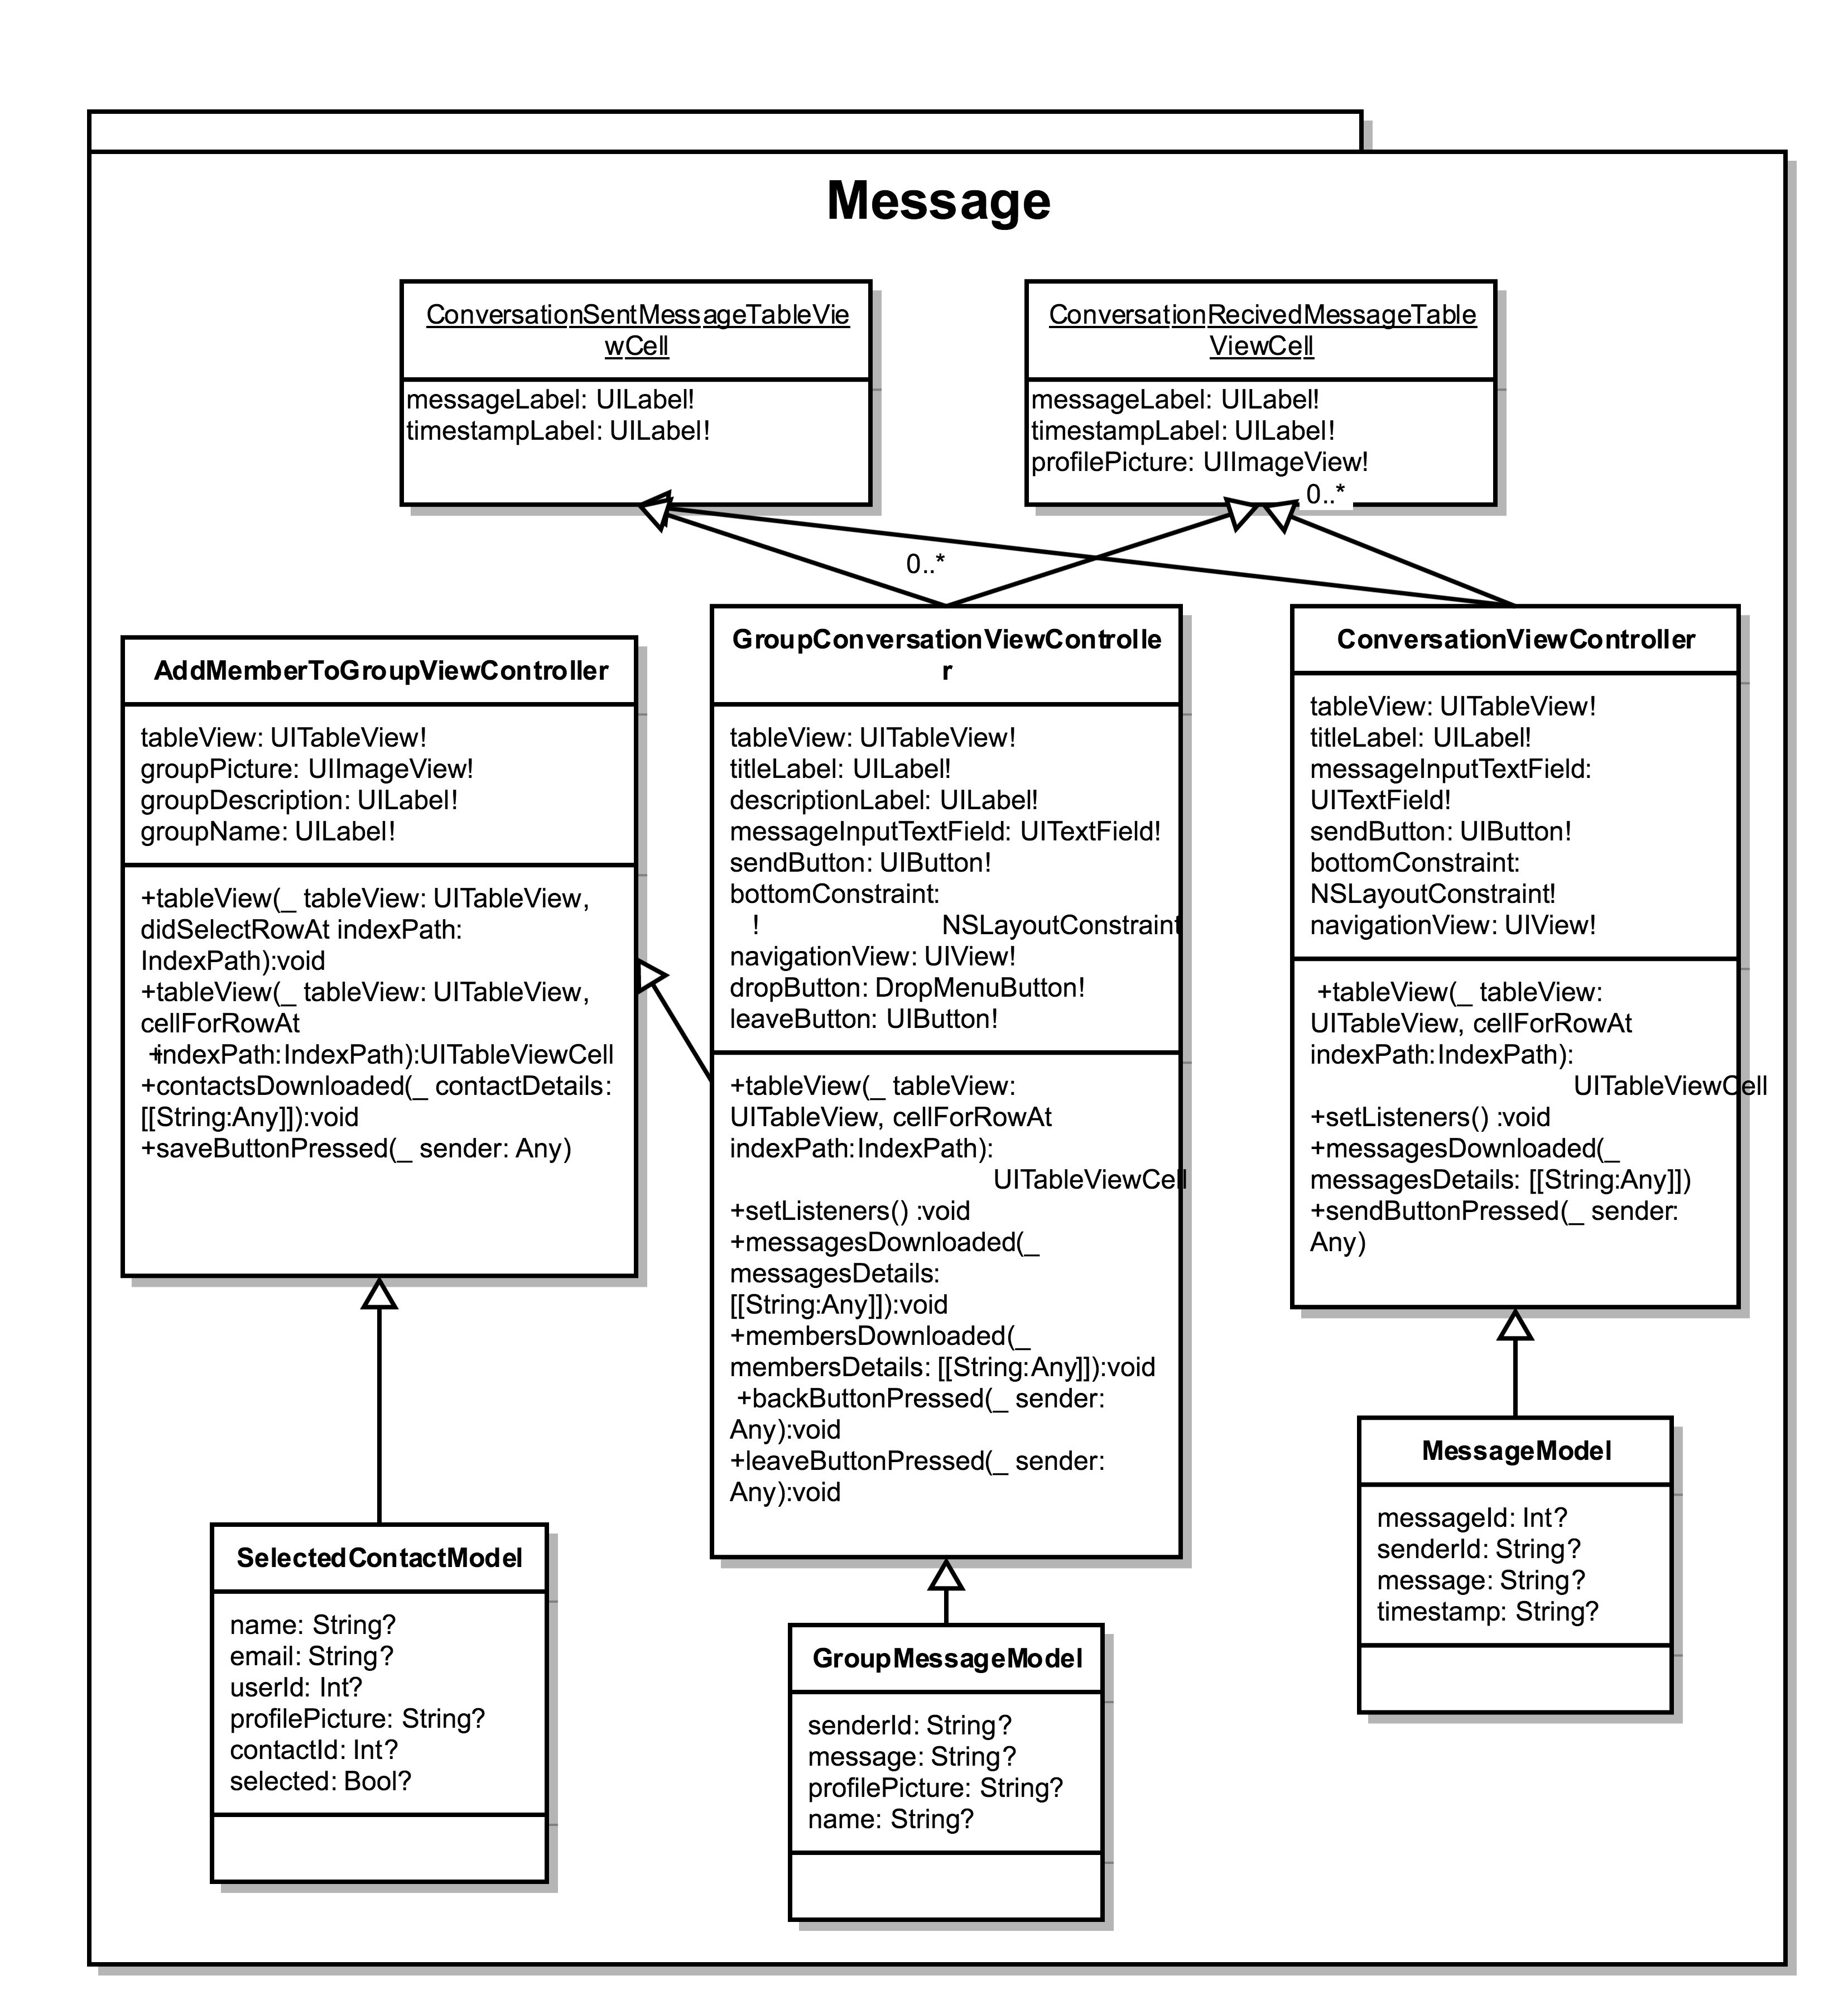
\includegraphics[width=.8\linewidth]{message.png}\hfill
		\end{subfigure}\par\medskip
		\caption{Example screen shots of Android's User Interface}
		
	\end{figure}
	
	Objects identified as Models encapsulate application specific data and define their processing logic. Most of the system's persistent data are managed using such objects. As Model objects define processing logic and do not have direct connections to the View objects, avoiding user interface shaping at this level, they can be easily reused in similar contexts. Such Models are the 'SelectedContactModel', the 'GroupMessageModel' and 'MessageModel' objects, which are reused in every conversation throughout the application, providing the means of storing and manipulating the incoming or outgoing messages, as well as contacts.\par
	
	User interactions that modify or create data by using the View layer are communicated through objects identified as Controllers and result in the creation or update of Modal objects. However, when such modifications are triggered either by receiving data through the network or by in-app events, Controller objects are notified in order for them to modify the appropriate View objects. For instance, View objects such as 'ConversationSentMessageTableViewCell' describe how sent messages should appear in the chat system's application. However, these objects are instantiated by Controller objects such as 'ConversationViewController', based upon the data stored in the 'MessageModel' Model objects.\par
		
	\subsection{\underline{\textbf{Web}}}
		\begin{enumerate}
		\item Class Diagram
		
		\begin{figure}[H]
			\centering
			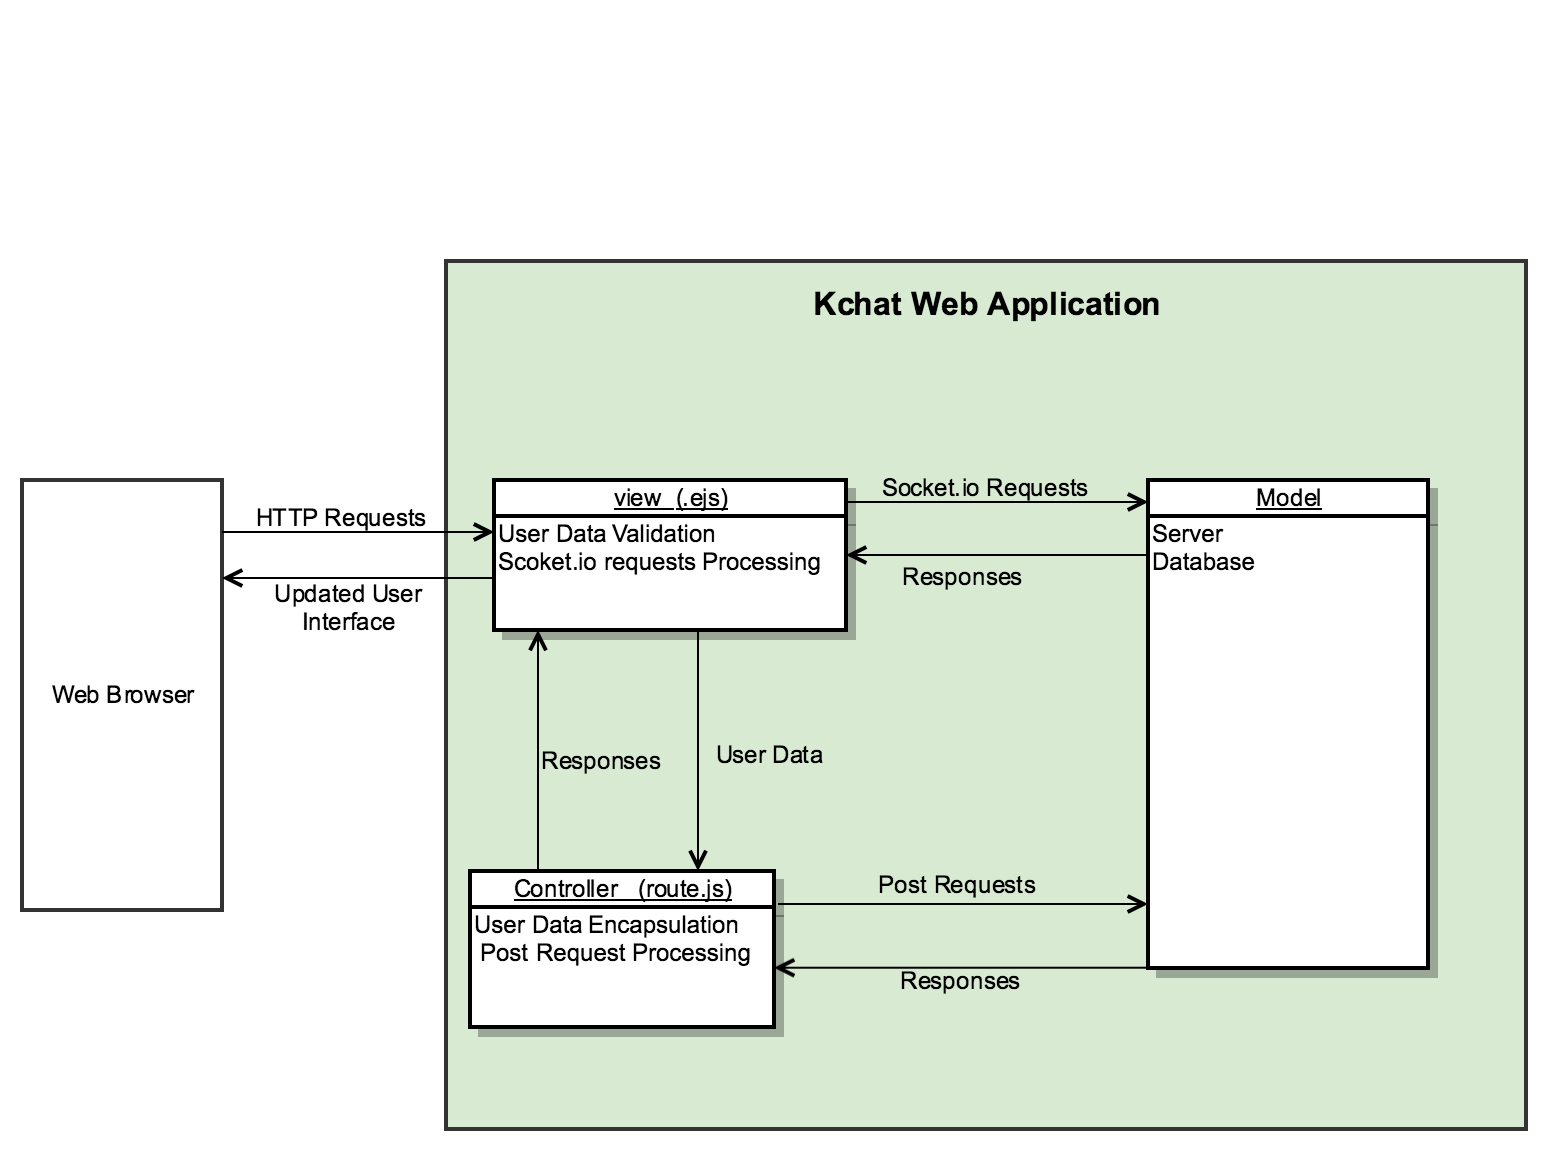
\includegraphics[scale=0.2]{webapp_architecture_diagram.png}
			\caption{Web Architecture Design}
		\end{figure}
		Figure 7 shows the Kchat web application applied to the MVC design pattern. The whole system is separated into three main components: View, Controller and model, allowing different ways of presenting information in internal system and to end user. \par
		\textbf{View:} As the component that displays all application user interfaces, this is where the data are presented to end user. Also, user events are collected here and interact with a controller to retrieve information accordingly. \par
		\textbf{Controller:} The component acts like an interface between view and model, as well as related high-level classes. This is where the user requests are handled and user data are manipulated for calling model component (in this case, server). Then, gather the response from the model and interact with the view to form the final output to end user. \par
		\textbf{Model:} The component defines the data structure of the application. In this application, the server acts as Model, as it receives all the requests from controller and interacts with database to retrieve or send data and pass the requested information back to controller for later use. \\ \\
		Advantages:
		
		\begin{enumerate}
			\item 
			Allows team members to work simultaneously on different parts of software. For example, one team member can work on the user interfaces while others can work on the controller part to define the business logic. This helps to boost the efficiency of software development.
			\item
			Reduce the work when changes happen, especially when changes happen on model part which does not depend on view, this enables us to modify the model part but no need to change the whole system architecture.
			\item
			Enables different ways of presentation information, because of the independence between model and view. This means that for one model we can have multiple views by defining different business logic rules in controller.
			\item
			Easy to understand, as the responsibilities of each components are clearly defined.
			\item
			Easy to debug, as the components are clearly separated so when an error appears in certain filed we only need to change the related component.
		\end{enumerate}
		
		Disadvantages: 
		
		\begin{enumerate}
			\item 
			Increase the difficulty of accessing data in views, as all the needed data in view has to be processed and passed by controller.
			
			\item
			Multiple developers are needed for developing the different components of MVC.
		\end{enumerate}
		
		\begin{figure}[H]
			\centering
			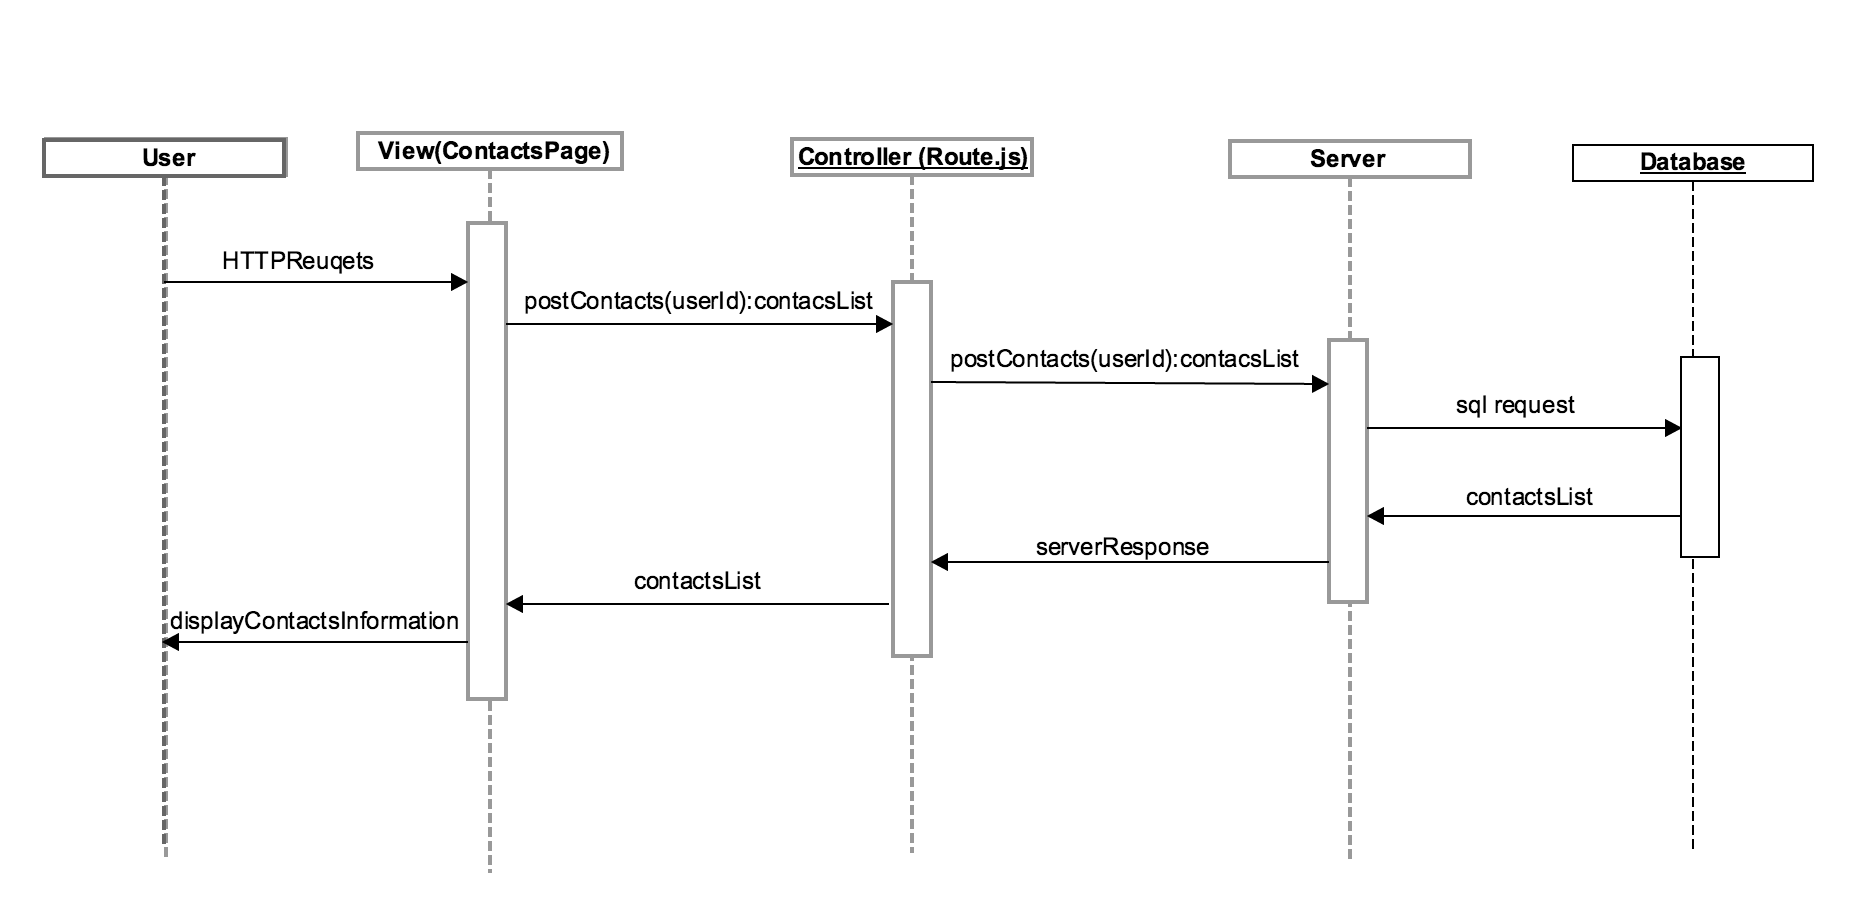
\includegraphics[scale=0.2]{web_sequence_diagram.png}
			\caption{Web Sequence Diagram}
		\end{figure}
		
		Figure 8 shows the complete process of how system handle specific user request with MVC flow. The process starts when user tries to access contact page, after which the page will send a post request with uerId as attached user data to handler. Receiving the user data, the handler will then try to connect to server using post request to retrieve information. Server, who acts as model in this case, will retrieve data from database and send back to handler who will then send the contacts information back to view. As a result, user can view the contacts information in the user interface. \\
		
		
		
	
	\section{Implementation}
	
	\subsection{Technology}
	
	\underline{Swift 3}\
	Swift is the most native and advanced language that people used to implement IOS application, which published by Apple in 2014 by using grammar dot-notation rather than the use of Objective-C pointers and other unsecured accesses. It is the newest vision which has more stable API, solving the problem of library changing by language improvement. Further removing Object C grammar such as “++” and loop ‘for’. As a coding language, Swift 3 combines the advantage from different coding languages that running with dynamic support, strict inspection in compiling and concise grammar. Basically, this is the most convenience and professional method in App development.\\
	
	\underline{Java}\\ 
	For Android mobile App, java is the most suitable method compared with the current main programming languages. Compared with the new languages, it has strongly library and steady platform. Although Java is not enough running efficiency compared with C++ and also less development efficiency than Python. At this stage of the mobile phone, the language should combine efficiency and cross-platform which effect on the consumption of power and app performance. In order to satisfy both of them, Java is the best selection now.\\ 
	
	\underline{Node.js} \\ 
	Depending on the event driven and asynchronous programming, Node.js can take full advantage of system resources and implement code without blocking. In server development, concurrent request processing is a big problem which can lead to waste of resources and time delay. Developers can improve resource utilization and performance through event registration, asynchronous functions. It is possible to run a number of Node.js processes, using certain communication mechanisms to coordinate the various tasks based on the multi-CUP.\\
	
	\underline{MySQL}\\
	MySQL server is one of the most widely used relational database management system, which strongly fixes the chat application needs because it is easy to use, with a rapid speed and high performance. As an instant message application, speed should be put high priority. Furthermore, MySQL is flexible open source which is the reason why it could be executed on all different platforms. In contrast, DoS attacks and spamming can wreak havoc on the database server, but it could be avoided by preventing performance issues and increasing uptime with a robust load balancing software.\\
	
	\underline{HTML/CSS/JAVASCRIPT}\\
	HTML, CSS, JavaScript are the best combination and a common method for web application development which also support distribute operating. Semantic HTML provides the pages’ structure; CSS implement the variability of style and make sure the interface professional and user-friendly. However, it also faces some problems. One of the biggest ones is the limitation of different browsers which result in some CSS or HTML format missing, but not a big issue.\\
	
	\subsection{Server}
	The server is a central component of the chat system, being in charge of the communication between clients and database, of the process logic and the conditioning of client's actions. Access to the persistent data is facilitated by MySQL queries on one or more tables, depending on the functionality that requests the data. The two-way communication between the clients and server is achieved and maintained by using Socket.IO. The data dispatch sequences are triggered by emitting requests upon certain listeners. For instance, in order to send a private message from a client, a request that contains specific message details is emitted on the listener "send\_chat" through the client's socket. The server is set to listen for this event on all of the sockets,performing an insertion in the database upon its receival and emitting the message through all of the sockets that listen to that particular conversation room. Thus, it ensures that the flow is correctly maintained for all the involved clients. \\
	
	Nonetheless, there were a number of difficulties in the implementation of the server. One of such problems was the double login.When a client's socket connected to the server, it was stored in an arraylist for future reference. However, if another instance of the same user connected to the server through another client's socket, it would have replaced the old instance. The problem occurred if the old instance would have then tried to perform more delicate actions such as sending a message. As the entry in the arraylist was replaced, the server would crash when trying to gather specific information from the new socket. The solution to this problem was to send a "disconnect" signal to the old socket before deleting its reference. Thus, the old client disconnected before allowing any new actions to be performed. However, the problem was not completely solved. If the old client loses internet connection while the server sends the disconnect signal, it reconnects upon internet connection, thus disconnecting the new user session.\\
	
		\begin{lstlisting}[language=Java]
socket.on('authenticate', function (userId, userFullName) {
  if (sockets["" + userId] != null) {
    sockets["" + userId].emit('disconnected', 'disconnect');
    delete clients[sockets["" + userId].id];
    delete sockets[sockets["" + userId].username];
  }
  socket.userFullName = userFullName;
  socket.username = "" + userId;
  clients[socket.id] = "" + userId;
  sockets["" + userId] = socket;
  socket.emit('authenticated', socket.username);
});
	\end{lstlisting}
	
	A second issue occurred when implementing the sending of messages. As the user interface shows sent messages with a timestamp,posting the actual time of when the message was received by the server was an issue. In case of a delay in sending the message,the sequence might have been corrupted, thus showing inconsistencies. This problem was solved by querying the database for the timestamp of the inserted message and sending it back to the client. However, this solution adds an extra query execution towards the database, overall adding a small, but constant overhead.\\
	
	Moreover, another problem occurred when trying to leave a group or when trying to delete the account of a group owner. As the tables in the database are functionally dependent on each other, the 'Owner' foreign key constraint from the 'Groups' table towards the 'Users' table would be broken. However, replacing the owner of the group with an anonymous user whose details are kept in the first tuple of the 'Users' table solved the problem. In addition, this approach inspired the idea of pointing the messages sent by every user that left a group to the anonymous user, thus preserving message consistency in the group.\\
	
		\underline{\textbf{Database}}
	
	Through the analysis of the system requirements, the database structure identified to provide the maximum degree of optimization for data storage is the relational database. Thus, the data was objectified and organized in tables, through identifying the purpose of every particular field. In addition, logical relations have been established between the tables, facilitating the extraction of complex information from the databse. As a result, the database structure for the chat system is represented in fig. x.\par
	
	The most important component of the database is the 'Users' table, which describes and stores the profile details of every user. As the system's main target is the communication between users, the 'Contacts' able provides the means to identify the connection between any two users. In addition, the 'Private\_messages' stores the messages sent between users, referencing the 'Users' table twice: once for the sender and once for the receiver. The functionality of creating groups has imposed the logical separation of the data stored for this purpose into an independent table 'Groups'. However, as a user can belong to several groups and more than one user can belong to a certain group, a many-to-many relationship is required, thus leading to the creation of the table 'Corelations', which serves the purpose of mapping the users to the groups they belong to. Finally, the table 'Group\_messages' stores the messages sent in every group, referencing both the 'Groups' and the 'Users' table.
	
	This structure provides the means to retrieve information in a seamless way. However, there were two situations in which more complex queries were needed in order to access the required data. As both the private and group chats windows need to display the most recent conversations ordered by the timestamp of the last message, retrieving these lists from the database implied combining the 'Users' and the 'Private\_messages' (or 'Group\_messages') twice based upon the 'senderId' and 'receiverId' foreign key constraints, selecting only the messages that have been sent between the two users ordered by the time of sending. This approach adds an inevitable, however small overhead to the retrieval of the chat lists.

	\subsection{\underline{\textbf{Android}}}
	\underline{User Interface}\\
	Implementing the user interface was not an easy step in the process. Android contains a series of components which look differently depending on the operating system version on the phone. One constraint faced was choosing which versions of mobile to support, for example supporting older mobile versions needed to include and compile a support library. the purpose of this support library is to replace new components with older components which are appropriate for the phones current operating system. This caused the user interface to look differently than intended so to solve this issue a decision has been made to target devices with an operating system of version 4.4 and above. More decisions have been made such as using Android Material Design, which is a library that contains a collection of themes appropriate for operating systems higher than 5.0 (lollipop OS). \\
	Once the correct version had been established it was then needed to implement the view which is responsible for representing the contacts and all the different types of chats. The original design was to use a list however this caused issues since only one design component could be inserted into the list which was not ideal since the requirements were also changed at this time to further display an contact image icon and more text to identify the contact. The solution was to use a recycler-view library which is a list that holds cards. Cards are a component themselves and are described as a panel which could hold many types of embeded components. One design instance of a card is used that contains two text fields and an image view. This can be seen in the appendix (figure 14). \\
	The functionality is defined by an adaptor where its purpose is to hold the relevant information defined as an Object arraylist. If data changes in the arraylist the adaptor updates using the notifyDataSetChanged method and then the recylcer would then re-set its adaptor.\\
	The issue was that the view was still not being updated this way and the issue was solved when the version number of the component was updated in android's dependency folder library.This problem was interesting to solve since there was no solutions to debug the component only by performing trial and error where one day was spent for this problem.\\
	
	\underline{Socket Communication}\newline
	Android makes use of the socket.io external library in the dependencies. One issue faced was that Android uses only one single instance of the socket in the whole project. This means that any new created socket instances will perform twice the operations and this problem was very difficult to debug, especially for detecting double sign-ins. The solution was to make the socket static and carefully hard-code exactly when to disconnect the socket (upon log-off) and when to connect.Testing was performed with log messages on the server and on the android side, the log contents were compared with the correct id's of messages to see if they matched. Issues were found since each socket that contains a .on() function would require an emitter from the server, meaning that there were many methods around that contained very similar names as connection prams to the server which made navigating through the code very difficult.\\ \\
	\underline{Rest Interface}\\
	One of the main issues in Android is identifying the two different types of threads. Android contains an UI thread that is responsible for compiling and creating the graphical components on the screen. Another thread is the background thread that is responsible for performing background operations such as communicating to the server via POST requests or performing work such as deserialising json's received from the server. One issue observed early on is that by trying to request the server in the UI thread would cause the application to crash or make the application run unresponsively.\\ The solution was to use Android background asyncTask which performs background information and publishes back the results from its work performed. One advantage of this is code-reuse for example the RESTApi class builds the complete POST request address and then sent to the server. \\
	\underline{Databases}\\
	Android uses a library interface that stores data in SQLite. Many issues were encountered since the team had no experience using SQLite nor its operations. During many hours of research and tutorial sessions spent on databases it was very difficult to observe the data contents in the database. In the end, stage data did get stored in the phones database for off line viewing and communication. \par
	
	\underline{Security}\\
	During the process of this project there were many security issues that were discovered and then rapidly fixed. One example is if a user was to log in and then log out, upon log out by pressing the back button would by-pass the login activity and then be directed to the previous users session where the new user has full access to all the previous user sessions functionality. To fix this issue the activity stack needed to be cleared and in the manifest file the activity login needed to have its history removed. Another security issue was notifications. If a user received notifications and triggered them via a tap would cause the app to force open to the activity where the notification was from. This was problematic if the user was not in the session and logged out. The problem was fixed by disabling the notifications intent navigation to not do anything on tap. One last security issue was data lifetime and database management. If a new user logged in the data was not cleared from memory or the database so the new user could use the previous users contacts and send messages. This was not ideal so the solution was to flush the databases and clear all contents from the arraylist.\par
	
	\underline{Constraints}\\
	Given the vast amount of requirements and their changes not everything could be fixed in time. Some of the most major issues shown above have been resolved both the issues that are to be mentioned now are bugs found which do not break the application but causes the application to function in a way as not intended from the begging. One example is the filtering problem where if a user contains a large list of contacts the filtering view shows correctly, however upon selection the item a different contact is shown. This filtering is performed on the chats and group layout screens.\\
	Another issue faced is the long wait to get the data in Json format from the server, since the server is not of a high performance type and is reasonably low cost, there was a wait of some time to receive the data. this also caused the application to wait for some time especially under heavy loads. The solution is to also be connected to a strong wireless Internet network to limit on the strain. More fixes could also be applied if more of the work was moved to the background thread so the user interface would show data however the background thread was at times working quicker than the UI thread so this resulted in putting the UI thread to wait for the servers critical information first. The last issue that was partly fixed was memory issues. If the user is using the application under heavy loads and wishes to download data then androids memory manager will complain and throw an error causing the application to crash. This is due to overflowing the allocated main memory in RAM. Solutions applied were to flush all databases and arraylist objects if the user logs out. A better optimal solution would be to implement database tables for each group or private chat.This would lastly increase the device stored memory and would be even more difficult to manage.
	
	\subsection{\underline{\textbf{iOS}}}
	
	
	\underline{User Interface}\\
	After identifying the required functionalities and defining the system's structure, the graphical interface was created in order to provide the users the means to use the iOS mobile application. The user-system interaction implies that the user reacts to the displayed information and the purpose of the design is to ensure a better user experience. In order to achieve this, the positions where the elements would need to be displayed was analyzed. According to Fitt's law, one of the fundamental principles of human-software products interaction, the time required to reach a target is a function based upon the distance and size of the target. In addition, the flow of the system has followed global principles, used in most chat applications.\par
	
	Another practice followed throughout the development of the mobile application is defining certain standards for the graphical elements. Thus, intuition is increased by the cognitive memory upon the visualization of elements with which users have already interacted. These elements have been created using View objects, based upon standardized purposes. For instance, the table cell objects used to display the contacts' information are reused throughout the application.\par
	
	\underline{System Structure}\\
	The implementation of the iOS mobile application did not come without difficulties. One time when the development process of the application was held up was in the case of uploading images from the device. Both the profile pictures and the group pictures are stored on the server using REST POST requests that contain the base 64 replesentation of the image. However, iOS requests automatically escape special characters, resulting in the corruption of the image string. The source of this problem was hard to identify as it seemed more likely that the issue resided in the conversion to base 64 or the conversion to JSON objects. As the iOS transmission protocols are very strict, there were no means of bypassing this problem in the mobile application. Thus, the solution found to solve this problem was to replace the empty spaces characters from the sent string back to '+' on the server.\par
	
	One interesting task from the implementation phase was storing the information locally for visualisation purposes in case of loss of internet connection. iOS provides a structure that allows storing data locally. However, the challenge was to save the more complex objects such as private and group messages (as well as information about the sender). This was achieved by setting encoding and decoding rules in the object classes and archiving the information upon retrieval. Then, when needed, they
	would be unarchived and presented to the graphical interface.
	
	The most important feature of the iOS application is sending messages. This in done by using the Socket.IO manager when internet connection is active. However,the mobile applications permit the users to send messages in an offline mode. As the recent conversations are saved, they are retrieved from the local storage upon entering a conversation window. When a user send a message with no internet connection, the local conversations are updated and the new messages are also added to a buffer, which is persistent for each user session. Upon reconnection to the internet, the buffer is flushed and sent to the server, which inserts the messages in the database.\par
	
	
	\subsection{\underline{\textbf{Web}}}

	\underline{UI Description}\\
			
	Figure 16 is a group chat view and can be accessed from url \\ http://188.166.157.62:5000/groupChat. The component of this page is
		
	\begin{enumerate}
		\item
			Header is contained the tab to change to another page such as the individual chat page, contact page, profile page. It also showing the logged in username and profile picture.
		\item
		Group chat page header is contained the create new group button, change group image button and a dropdown with submenu leave group, invite others to group and delete group.
		\item
		Group chat list is located in the left side of the page and will showing all of the group list and recent message.
		\item
		Group chat room is located in the right side of the page and will showing the message content of the selected group chat.
		\item
			Send message part is located at the bottom of the page. It is contained the text field and send button. This part is where the message will be typed and sent.
	\end{enumerate}
		
	Figure 17 shown a contacts page view and can be accessed from url \\ http://188.166.157.62:5000/contacts. The component of this page is
		
	\begin{enumerate}
		\item
		Three tabs at the top of the contact page is showing the contact request sent, received contact request and search a user to be added.
		\item
		Search contact list is the component we can search our contact list.
		\item
		Contact list is located below the search contact list and showing all of our contacts.
		\item
		Contact profile is located at the right side of the page and will showing selected contact’s details. There is a delete button and start conversation button for each contact.
	\end{enumerate}
	
	\underline{Problems}\\
	
	\begin{enumerate}
		\item 
		The different type of data which sent from and to the web server:
		
		In this part, we face a problem where the web server data is formatted in string and the web view part is formated in JavaScript Object Notation (JSON). To handle this implementation, we are using JSON to exchange the data. So we are using json.parse() to parse the json image data or javascript value from the view to the server side. This method parses a JSON by constructed the image or object described by the string. json.parse() also support nodejs. Example of using the JSON.parse():
		
		\begin{figure}[H]
			\centering
			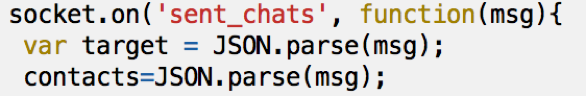
\includegraphics[scale=0.6]{problemWeb1.png}
			\caption{Example of JSON.parse()}
		\end{figure}
		
		Figure 9 is the example of using JSON.parse() syntax in the sentchats function to parse the data in variable msg to the variable target in order to make it readable for javascript.
		
		\item 
		Parsing the chosen contact userid to start a conversation:
		
		In this part we want to open a new chat box at individualChat.ejs based on the start conversation’s button in the chosen contact in the contacts.ejs view.
		In order to dealing with this problem, we adding a new function in the controller routes.js to get our chosen contact’s id and name then process it to open the individualChat.ejs page to make a new chat list for the targeted name.
		Code example:
		
		\begin{figure}[H]
			\centering
			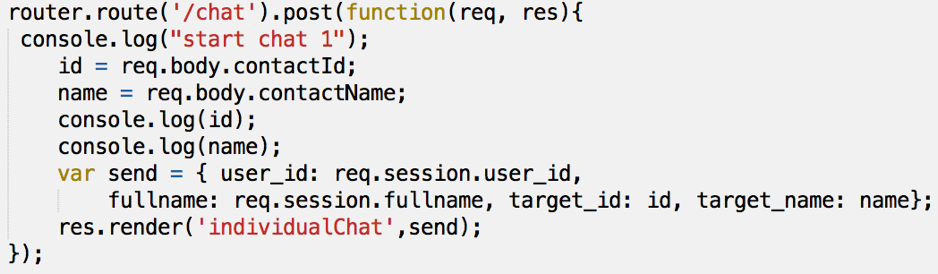
\includegraphics[scale=0.4]{problemWeb2-1.png}
			\caption{routes.js}
		\end{figure}
		
		Figure 10 is the function in controller to open the individualChat.ejs view and parsing the variable send.
		
		\begin{figure}[H]
			\centering
			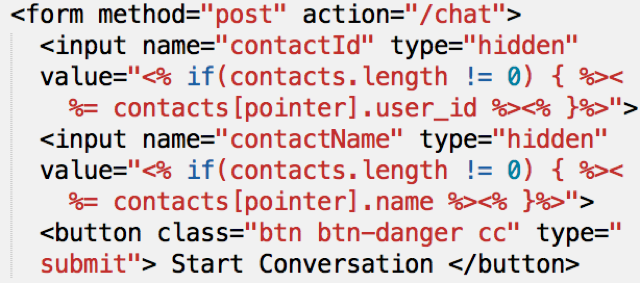
\includegraphics[scale=0.4]{problemWeb2-2.png}
			\caption{contact.ejs}
		\end{figure}
		
		Figure 11 is the action if the user clicked the Start Conversation button. So it will open the chat function in the controller with the value of contact userid and contact name.
		
		\item 
		Socket io in the server does not cover all the information provided in the database about group member:
		
		In this part, we need to show the username and message in the chat box, meanwhile the table which contain the message only has the user id of the sender of the message. In order to show the username, we made another function as shown in the figure 12.
		
		\begin{figure}[H]
			\centering
			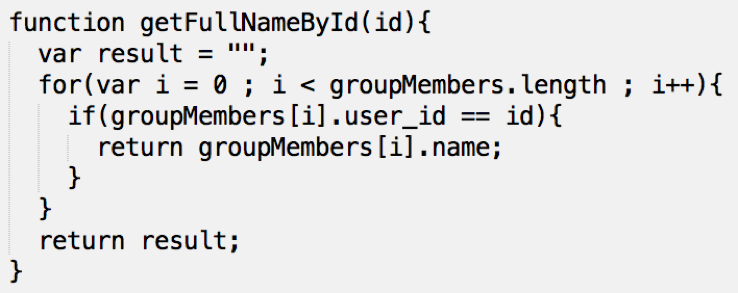
\includegraphics[scale=0.4]{problemWeb3-1.png}
			\caption{Function to get the username}
		\end{figure}
		
	\end{enumerate}

	\newpage
	
	\subsection{\underline{\textbf{Testing}}}

	One testing methodology used in android is component testing. This methodology involves separating components of the system and testing their provided interfaces. Their behavior is observed to record if the component performs its function as intended. Mostly UI components have been tested by adding data to them and measuring many components can be shown on the screen at the time. This testing methodology has helped to solve the issue of displaying messages since if more than 30 messages are to be displayed on the screen would make the phone crash. The decision was then to limit the number of messages on the screen to just 20.\\

	Another testing methodology used was performance testing. This methodology observes how the mobile device performs under the applications functionality. Observations such as the memory status levels, amount of data required to obtain data and the time it takes to receive the data back from the server. By observing figure 19 in the appendix we could see that the blue diagram represents the main memory levels, orange is the network level over time and red represents the levels of CPU processing and calculations. From these tests any abnormal levels were recorded during operating the application such as discovering that if another user logs in a session the memory was not cleared so the application crashed, from these charts we fixed this issue on the mobile device.\par

	For Web Application, we did system test for testing all the critical features of kchat, and following are the testing records at March 28th, 2017: \\
	
	Test case: user can access the websites with common web browsers  \\
	Test description: User can access to any of the web pages with common web browsers (google chrome, Firefox , opera,safari , IE, ) \\
	Excepted result: System displays the web pages with correct information and in order \\ 
	Pass/Fail: Pass \\
	
	Test case: Login \\
	Test description: User can login with correct username and password \\
	Excepted result: System redirect to individual page with user’s chat list \\
	Pass/Fail: Pass \\
	
	Test case: user can open the chat content \\
	Test description: In individual chat page, user can select one of the available chat list and see the chat content in the chat room \\
	Excepted result: The selected chat list showing the chat content in chat room \\
	Pass/Fail: Pass \\
	
	Test case: user can start individual chat \\
	Test description: In individual chat page, user can send a message to the selected chat list \\
	Excepted result: The message appears in chat room and another client receive the message \\
	Pass/Fail: Pass \\
	
	Test case: user can open the group chat content \\
	Test description: In group chat page, user can select one of the available group chat list and see the chat content in the chat room \\
	Excepted result: The selected group chat list showing the chat content in chat room \\ 
	Pass/Fail: Pass \\
	
	Test case: user can start group chat \\ 
	Test description: In group chat page, user select one specific group, and send message \\
	Pass/Fail: The message appears in group chat room and other users in this group receive the message \\ 
	Pass/Fail: Pass \\
	
	Test case: user can create group \\
	Test description: In group chat page, user can create group by entering group name, group description and choose group member \\
	Excepted result: The group appears in the group list and members of this group can start to chat in the group room \\
	Pass/Fail: Pass \\
	
	Test case: user can view contacts information \\
	Pass/Fail: In contact page, user can view the contacts information as well as delete and add contacts \\
	Excepted result: The contacts information display in the contact page accordingly \\
	Testing Result: Pass\\
	
	Test case: user can start conversation with new contacts who he never chatted before   \\
	Test description: In contact page, user can start conversation with a contact he never chat before \\ 
	Excepted result: The system redirect to the induvial page with the contact selected appears in the top of the chat list \\
	Pass/Fail: Pass \\
	
	Test case: user can view chat list \\
	Test description: In private chat and group chat page, user can view the lists of chats he ever had before \\ 
	Excepted result: System display the private chat list or group chat list in private chat page and group chat page respectively. \\
	Pass/Fail: Pass \\
	
	Test case: user can register account \\
	Test description: In register page, user can register new account by entering required information \\  
	Excepted result: System redirect to individual page with the newly registered user information \\
	Pass/Fail: Pass \\
	
	SERVER\\
	Test case: deserialize Json for contacts\\
	Test Description: deserialize a json object to  a string format then store in the database based on tags\\
	Expected result: stored in the appropriate location in the database columns based on the json object tags\\
	Pass/Fail: Pass\\
	
	Test case: test connection to the server\\
	Test Description: send a string message to the appropriate link as a post request\\
	Expected result: receive the post request and reply back to the device with a string message\\
	Pass/Fail: Pass\\
	
	Test case: validate double sign-in requests\\
	Test Description: check the conditions of the socket on the server and if there is a duplicate socket id for the room then reply back to the device.\\
	Expected result: mobile device received the message to sign out rapidly\\
	Pass/Fail: Pass\\
	
	Test case: extract client data from servers database\\
	Test Description: Test the appropriate SQL select statement and print back the result of the request\\
	Expected result:The process took longer than expected to obtain the data, the query need to be modified to function optimally\\
	Pass/Fail: -\\
	
	IOS\\
	Test case: observe notification behaviour\\
	Test Description: The notification should play a sound and show a design panel with appropriate text\\
	Expected result: shows the notification first time and plays the appropriate sound\\
	Pass/Fail: Pass\\
	
	Test case: send message to the server and print on the screen any received messages\\
	Test Description: The server should receive the message and store its contents, any new messages should be shown on the device's UI\\
	Expected result: The message is sent to the server and the server replies back with any other new possible messages, the messages are displayed on the screen\\
	Pass/Fail: Pass\\
	
	Test case: force sign out on double sign in\\
	Test Description: wherever the user is in the application if the server replies back with a double sign in then the user should be forced to leave the application and be directed to sign in.\\
	Expected result: the user did get signed out and rapidly moved to the login page upon server's response.\\
	Pass/Fail: Pass\\
	
	Test case: test the clients session on the phone\\
	Test Description: test that the user is still in session if the application has been put in the background, resume the session until log-out.\\
	Expected result:The user did not get placed back into the log in screen, sessions function correctly\\
	Pass/Fail: pass\\
	
	Android\\
	Test case: observe image upload\\
	Test Description: The user should upload his profile image to the server and then it should update on the screen for the users profile.\\
	Expected result: image is sent to the server and stored in the appropriate place, the android device shows the correct users profile\\
	Pass/Fail: Pass\\
	
	Test case: change contact details\\
	Test Description: the contact should hold tap the labels on the contact page, modify them then the correct data should be sent to the server.\\
	Expected result: the server receives the data for each type of label and updates the information on the device\\
	Pass/Fail: Pass\\
	
	Test case: filter contacts correctly\\
	Test Description: filter contacts depending on the text entered in the edit text component.\\
	Expected result: the view re-refreshes and shows the correct cards but upon selection displays the incorrect card.\\
	Pass/Fail: Fail\\
	

	
	\subsection{Licences}
	During the course of this project software libraries have been taken from other sources. No modifications has been made to any libraries taken nor do we obtain its full rights as owners. One library taken was socket.io which has been used for the main communication channel which was vital to our work Another library used is android material design by Google which was used to customize the views of the android mobile device to give an elegant appearance . Express js was used for embedding javascript into HTML for the web platform. Jquery, Font-Awsome, and brainhadaway, jqueryModal, Bootstap for styling the web UI. Json Api for data handling on the web side part for working with jsons. Swift3 and  iOS Drop Down Menu has been used for iOS development and styling. Finally we used technologies from SQLite and PHPmyadmin for the mobile and server side data processing.
	
\end{enumerate}	


\section{Team work and group management}

Time restricted projects successfully require adaptive development methodologies and well-organized teams. It is important to implement functionalities in the order of decreasing priorities to meet a deadline. In order to achieve the purpose, we adopted Agile software development process because it reduces the risk for delay by splitting the whole implementation process into small cycles with each functional priority. In addition, efficient project progress demands close collaboration among team members because it is a key element to eliminate duplicate works and crucial problems in project progression. Therefore, we have also utilized various communication tools among team members not only to share progress but to work collaboratively with other mates.        
\subsection{Agile methodology}
Agile software development process provides notable features to achieve time restricted projects. Especially, the implementation phase that accounts for the majority of software development projects is accelerated because sequential process, such as requirement definition, design,  implementation, testing and code review, is achieved by iteration with short-term cycles. Moreover, software development based on this model realizes implementation of high priority functionalities in early stages compared with traditional methodology represented by Waterfall model which commences implementation of applications after complete definition of all requirements.\\      

\begin{figure}[h]
\centering
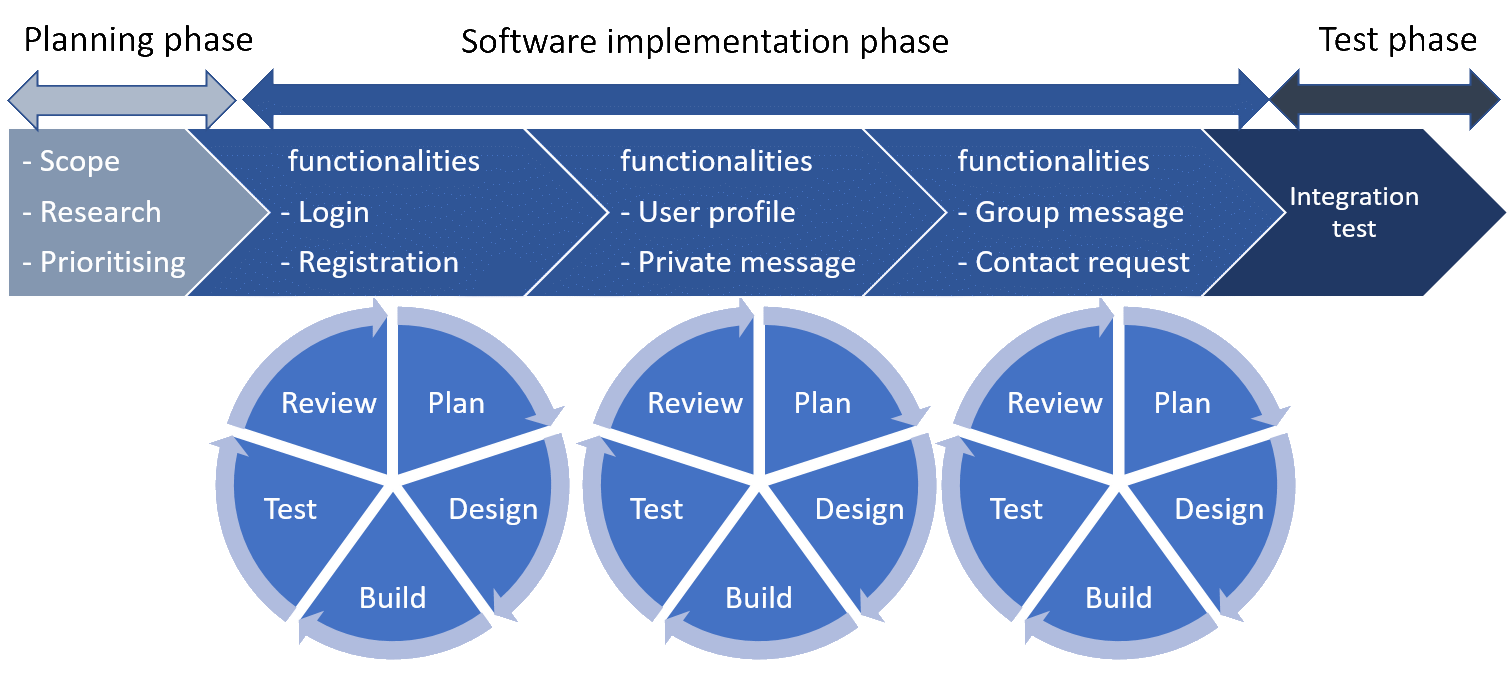
\includegraphics[scale=0.3]{agile.png}
\cite{agile}
\caption{Development process based on Agile methodology}
\label{fig:agile}
\end{figure}

Our project is divided into three major phases. Firstly, we built the plan to implement preferentially to high priority functionalities. Secondly, based on the Agile model, we addressed software implementation phase which consists of three short-term cycles with priorities. Finally, our software comprised of outcomes in each cycle was tested. These development flow is shown in Figure \ref{fig:agile}.

\subsubsection{Planning Phase}
At the beginning of the project, we discussed comprehensive scope and direction that Android, iOS and Web are necessary as clients platform for large coverage. In addition, on the assumption that Agile is the optimal model for this project, team building led to the balanced assignment of members composed of the experienced and inexperienced person in each platform through respecting for individual intention. Moreover, we decided to research state-of-the-art technologies to achieve real-time chat system with our own viewpoints. \\
Findings based on individual research provide the result that node.js and socket.io are suitable for this project. However, we were faced with a significant problem that all the members were complete beginners for those technologies. To address this issue, we dig deeply into them by sharing information such as the introduction of demonstration video. Consequently, we successfully prioritised key functionalities based on global perspectives for this project.
\subsubsection{Implementation Phase}
We divided implementation phase into three parts with priorities according to Agile methodology. First, the highest priority was assigned to login and register functionalities. Second, user profile information and individual chat were regarded as preferential activities because these support fundamental functions of the project outcomes. Finally, in order to construct more attractive chat system, we decided to implement contact requests for individual users and chatting page for groups.\\
Through all the implementation phases, the experienced person not only made efforts to obtain further complicated techniques but actively provided another member with beneficial information to master programming skills as soon as possible in each platform. On the other hand, the inexperienced person also dived into novel field without overly concerned about unknown technologies.\\
The members of each team collaboratively built plan, created design, wrote codes, conducted unit tests and pushed them for review. In addition, design consistency was kept through meetings beyond the bounds of each team.       
\subsubsection{Test Phase}
Implementation phase was followed by integration tests to check the proper and stable behaviours of all the functionalities. Especially, not only communication between the server and clients but page transitions between functions which were implemented on different priorities were tested. Performing such tests resulted in maintaining data and page consistency on cross-platform environments. 

\subsection{Tools}
In order to perform effective Agile methodology, all the members are required to build close connection each other. This is because launching functionalities in short-term are supported by mutual understandings among members. For example, when a member is facing with some problems, speedy situational awareness is required to avoid delay of the project. We utilised a variety of tools to grasp members situation and progress.           
\subsubsection{Face to face}
Face to face interview is the most effective method to aware abnormal circumstances although it is rapidly regarded as legacy way. We have aimed to meet up and consult individuals. As a result, such attitude has incubated recognition of the importance on each member. Hence, we successfully accomplished our project with various sophisticated functionalities within the deadline. Especially, without face to face meetings, we could not conduct complicated discussions such as parameters between server and clients, design consistency and page transitions.\\
On the other hand, it is the fact that we had missed some opportunities to meet up. We have utilised not only physical contacts but a variety of online tools such as Trello, slack, facebook and skype. The combination of these tools is essential to building close communication between individuals.
\subsubsection{Online tools}

Trello \cite{trello} is effective tool to record backlog with priorities and to check progress on each task. Each member enables to grasp not only own remaining tasks but other members ones. Therefore, we have utilised this tool to keep constantly members workloads by assigning works appropriately.\\

Information sharing is the most important element to unite project members. We have employed Slack \cite{slack} to share data and situation. For example, chat page design, informative video and error messages on the server were shared through Slack. Moreover, we have provided various granularity information not only all the project members but individual one.\\

Cooperative software development is supported by version management tool such as Git\cite{git}. We have utilised Git and Git Hub to keep latest codes and refer update histories in our team. Particularly, we have managed adaptive branches in response to the implementation phase. In the end, we have performed approximately 400 commits to Git and this has led us to the achievement of the group project.\\
We have also utilised Facebook and Skype. The former was used to grasp the situation and pleasure regarding each member. In addition, we have employed the latter as a visual communication tool instead of difficult face to face meeting. Especially, Skype was significantly useful to share the display of the member when instructing another person.



\section{Evaluation}


	Over the course of this project as a team we had strong agile team management methodologies that were established from week 1. This allowed us to use online management tools which were necessary for keeping track of our projects backlog. As a team we worked really well as pair programmers, we helped one another across teams and would meet up as regular as possible. Together we worked well on solving the most highest prioritized tasks first on time. The team worked excellently debugging and solving each others issues. The team tried really hard to follow the time line of the roadmap produced earlier but due to unforeseen circumstances it appeared to be very difficult to follow. One issue was illnesses to a couple of team members which resulted in the work being behind schedule by 2 weeks. It was even harder to catch up to the work. This further resulted that some of the less important features such as image upload could not be completed as well as encryption on the message stream. None of the team members complained about the work given and some plans needed to be changed or drop-ed, other members were required to take up more work for themselves or solve their current work faster.\par
	
	Realistically as a team given the timescale and each other members busy schedules we could never produce a professional style chat application. As a team our weakness were mostly working across platforms where we would sometimes overwrite each others code on the cloud server. Time has been spent to find backups of the work and reload the server to a previous state.\\
	
	If your team had been given more time we would have enjoyed to solve some of the more difficult implementation issues such as:
	
	\begin{enumerate}
		\item Implementing the upload image functionality where images are to be stored in a database.
		\item Allow encryption of messages over a stream where messages are to be encrypted using a strong encryption mechanism such as blowfish with salting for stringer protection.
		\item Include admin functionality, especially for the web part where the admin would have a panel to block or remove accounts.
		\item Implement a faster noSQL data store on the server such as Firebase where querying is performed faster and less maintenance is required to uphold.
	\end{enumerate}

To evaluate during the whole process we each have gained new skills in programming, communication and self confidence when solving problems. this module has helped us to behave professionally in the real world and tackle issues differently. This was all gained from learning from one another and repairing our weakness to be better team members.

\section{Peer assessment}

The team has established that the peer assessment should be done democratically. Each team member had 100 points to divide in between the teammates, as well as to himself/herself.As the team worked closely toghether in the development phase, with daily meetings and access to the github repository, each member had a good idea of everyone's contribution. Thus, based upon individual criteria, the team coordinator received the grades, calculated the average for each teammember and divided by 6. Thus, the results were: \\


Yuke Chen        14.56\\
Yixiang Gong     12.55\\
Tiffani Rachman  10.56\\
Kensuke Tamura   15.23\\
Tudor Vasile     23.55\\
Tudor Zugravu    23.55\\ 
\section{Appendix}
\begin{figure}[H]
\begin{subfigure}{\linewidth}
		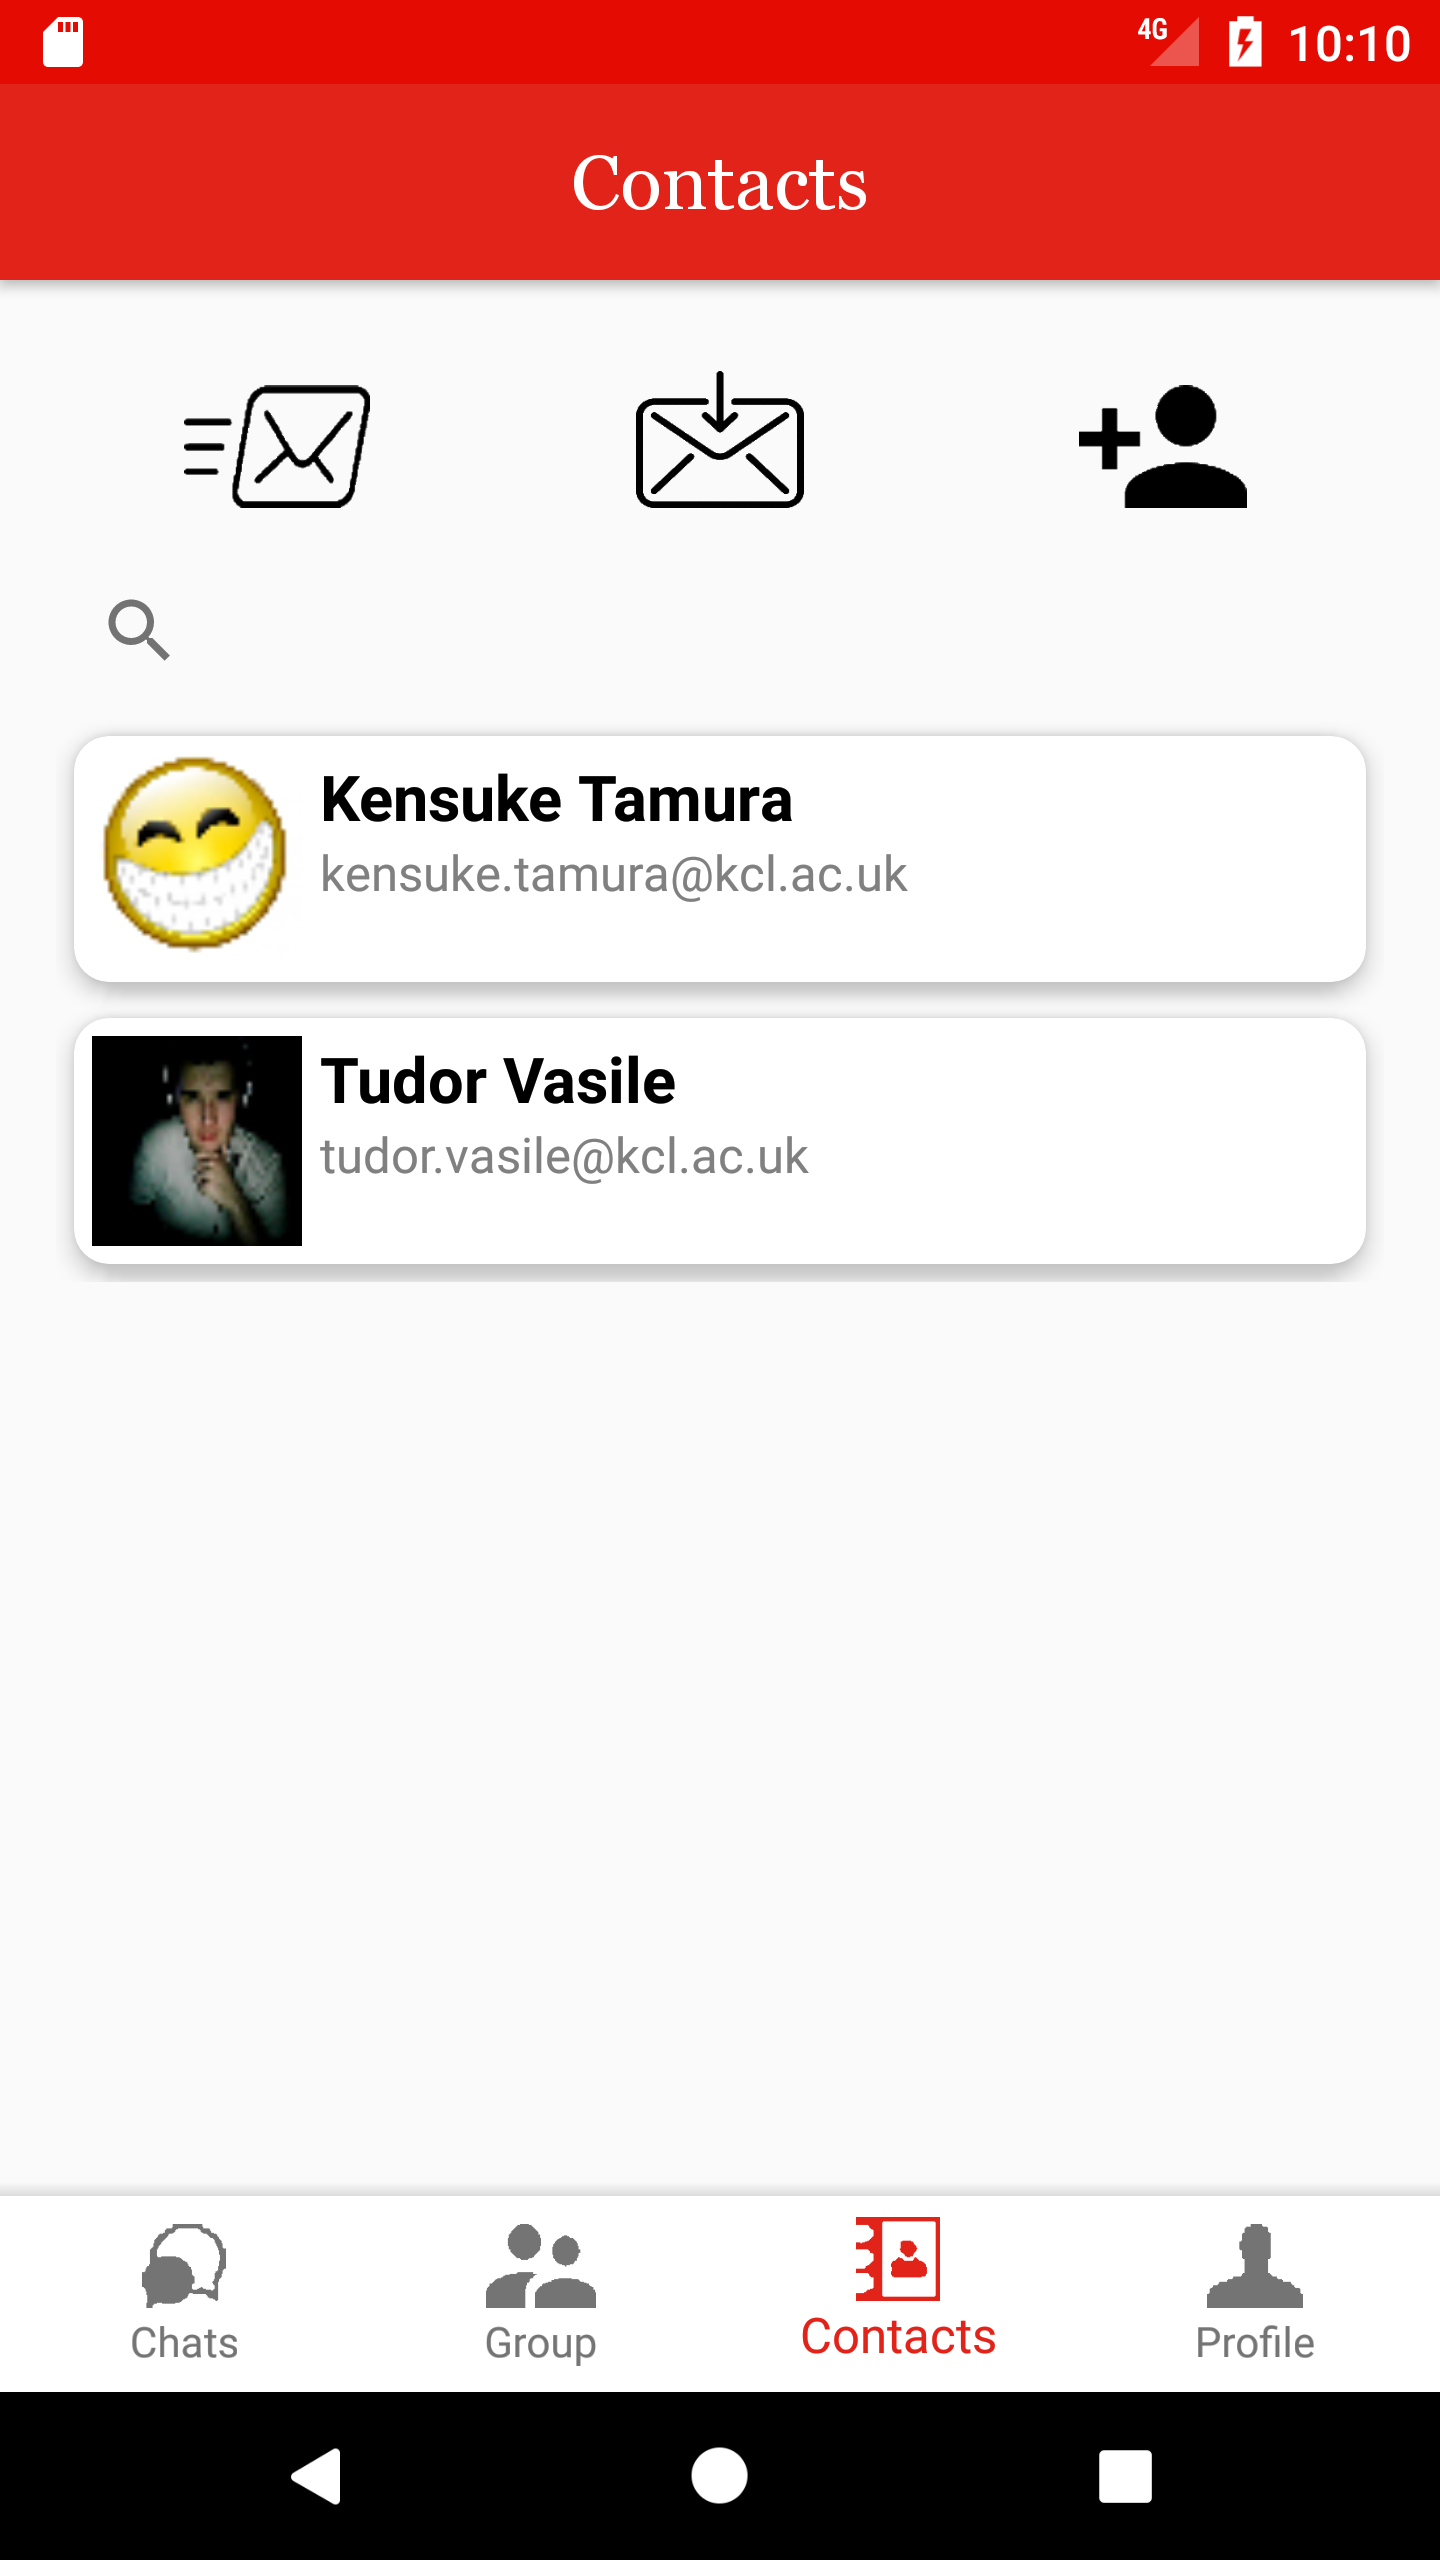
\includegraphics[width=.3\linewidth]{contact_list.png}\hfill
		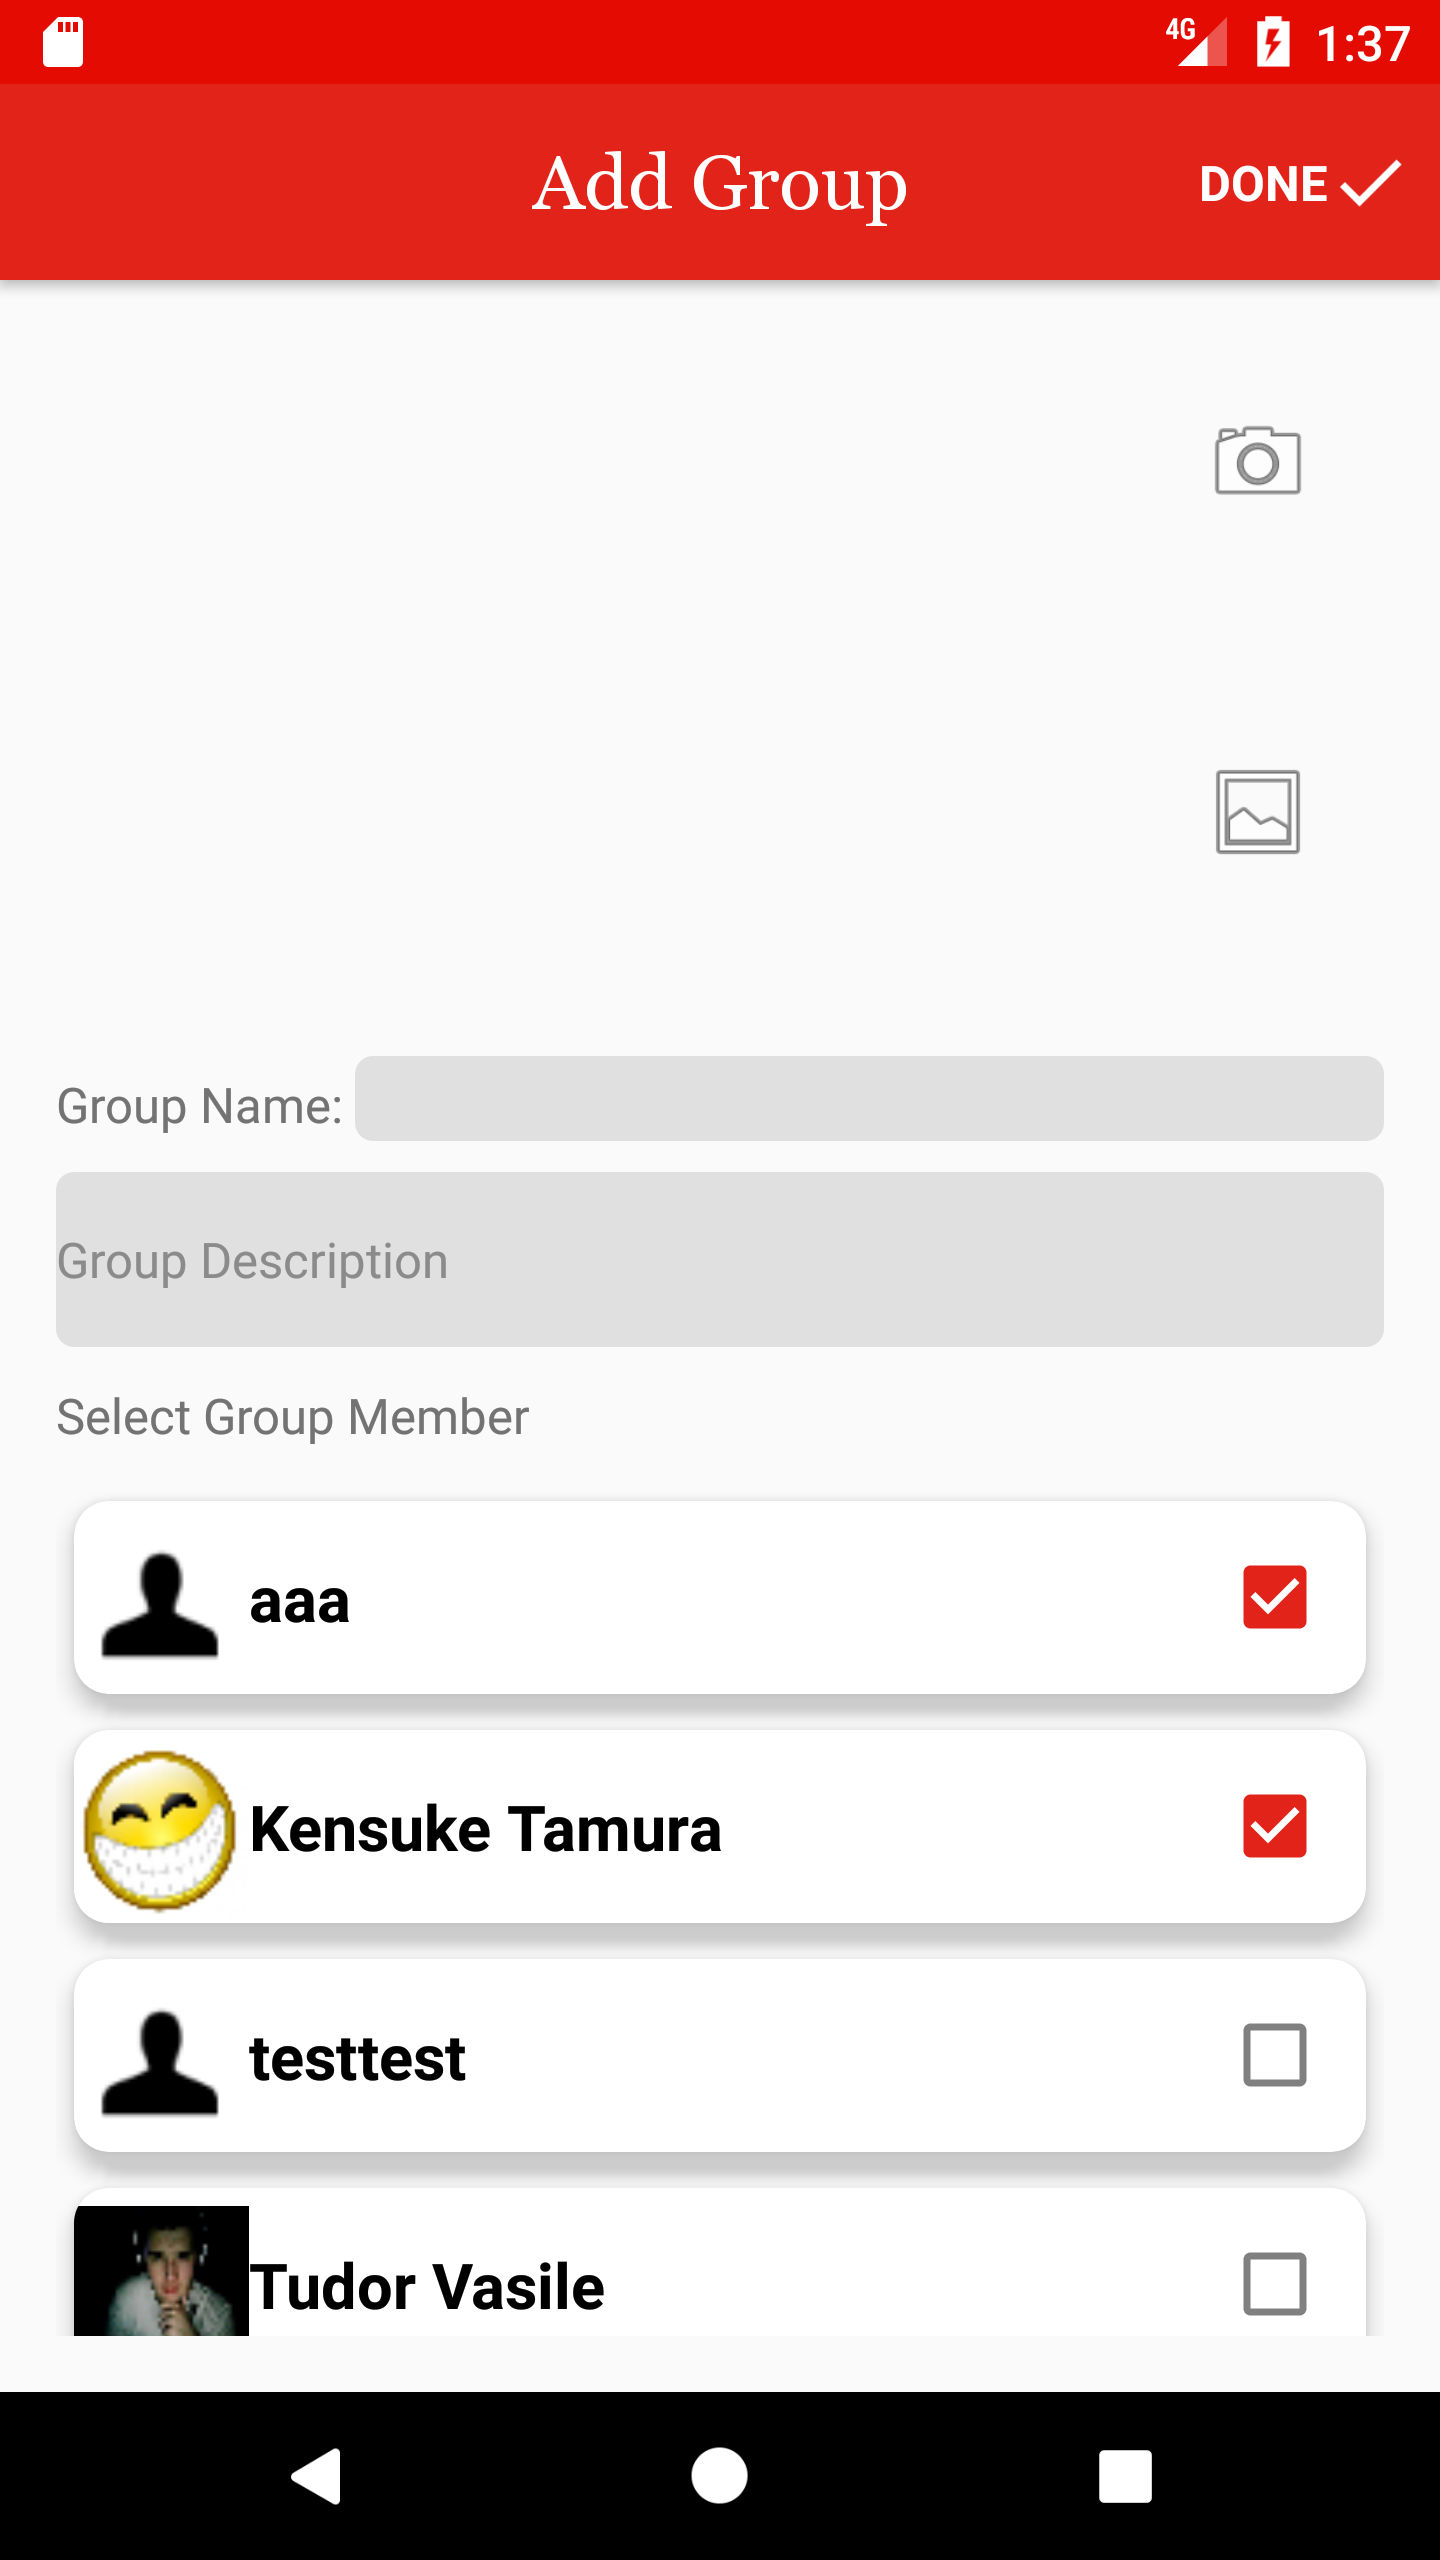
\includegraphics[width=.3\linewidth]{add_group.png}\hfill
		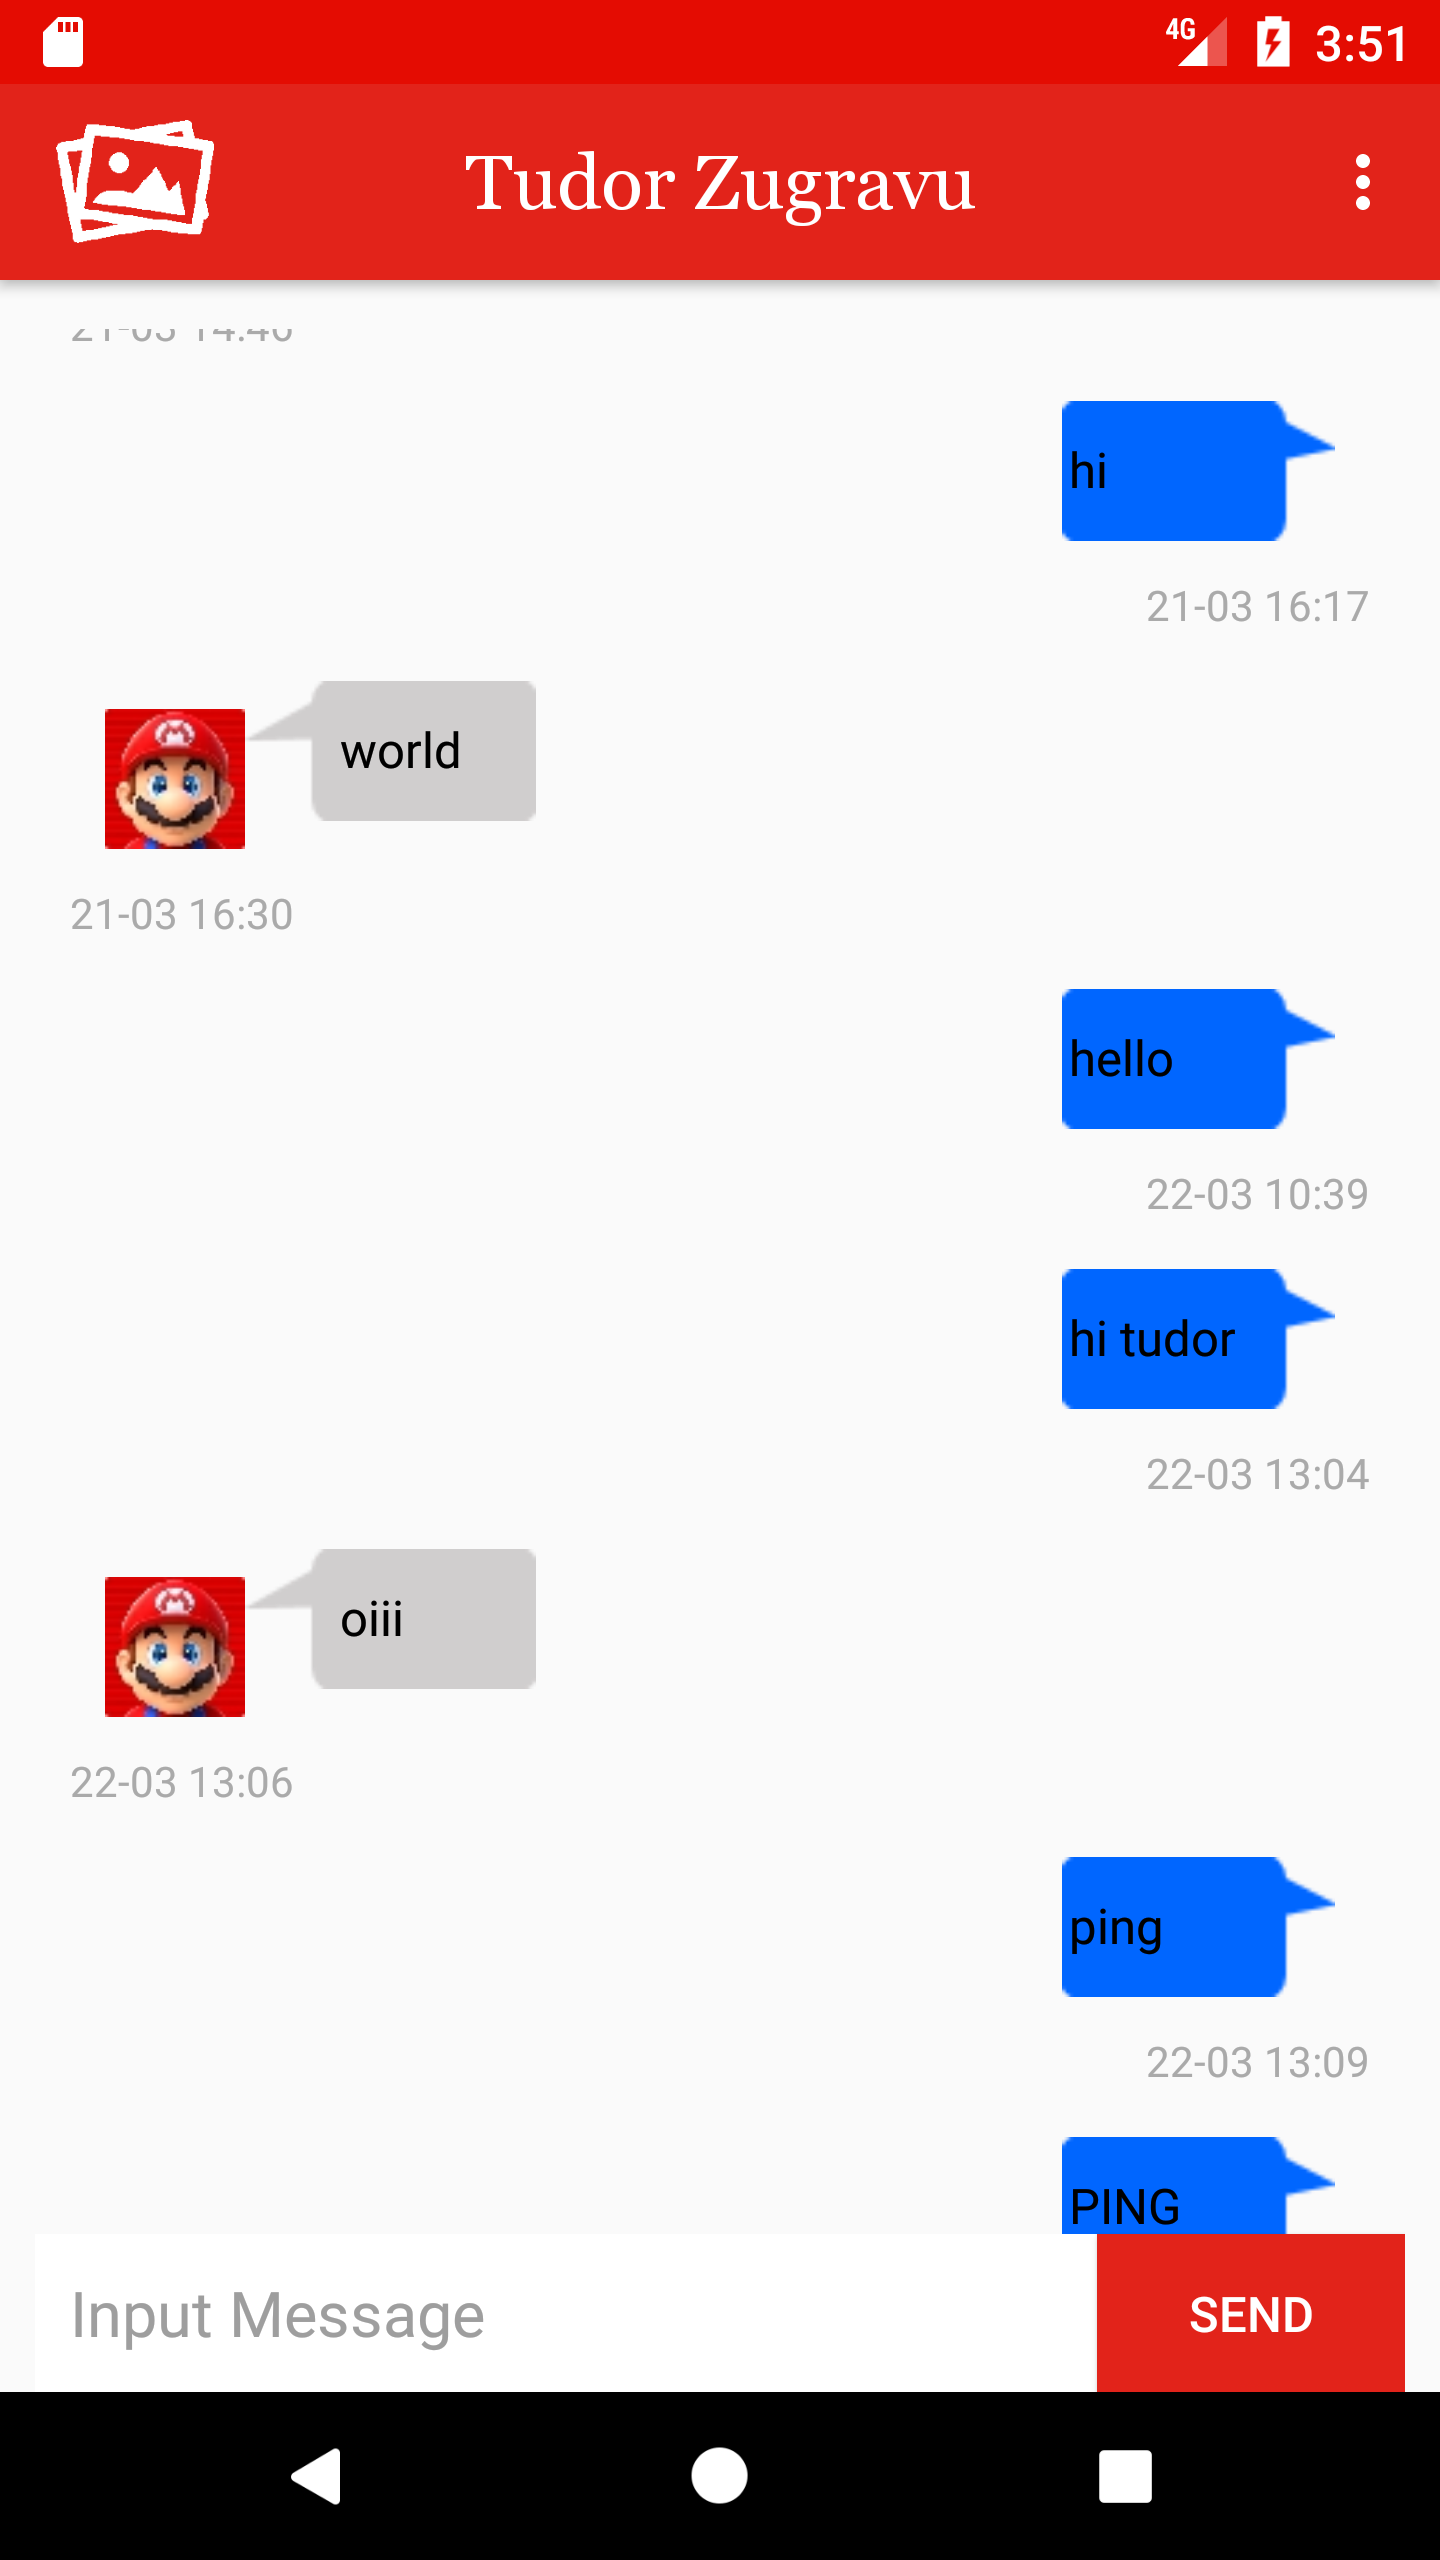
\includegraphics[width=.3\linewidth]{chat_page.png}

\end{subfigure}\par\medskip
		\caption{Example screen shots of Android's User Interface}
\end{figure}

\begin{figure}[H]
	\begin{subfigure}{\linewidth}
		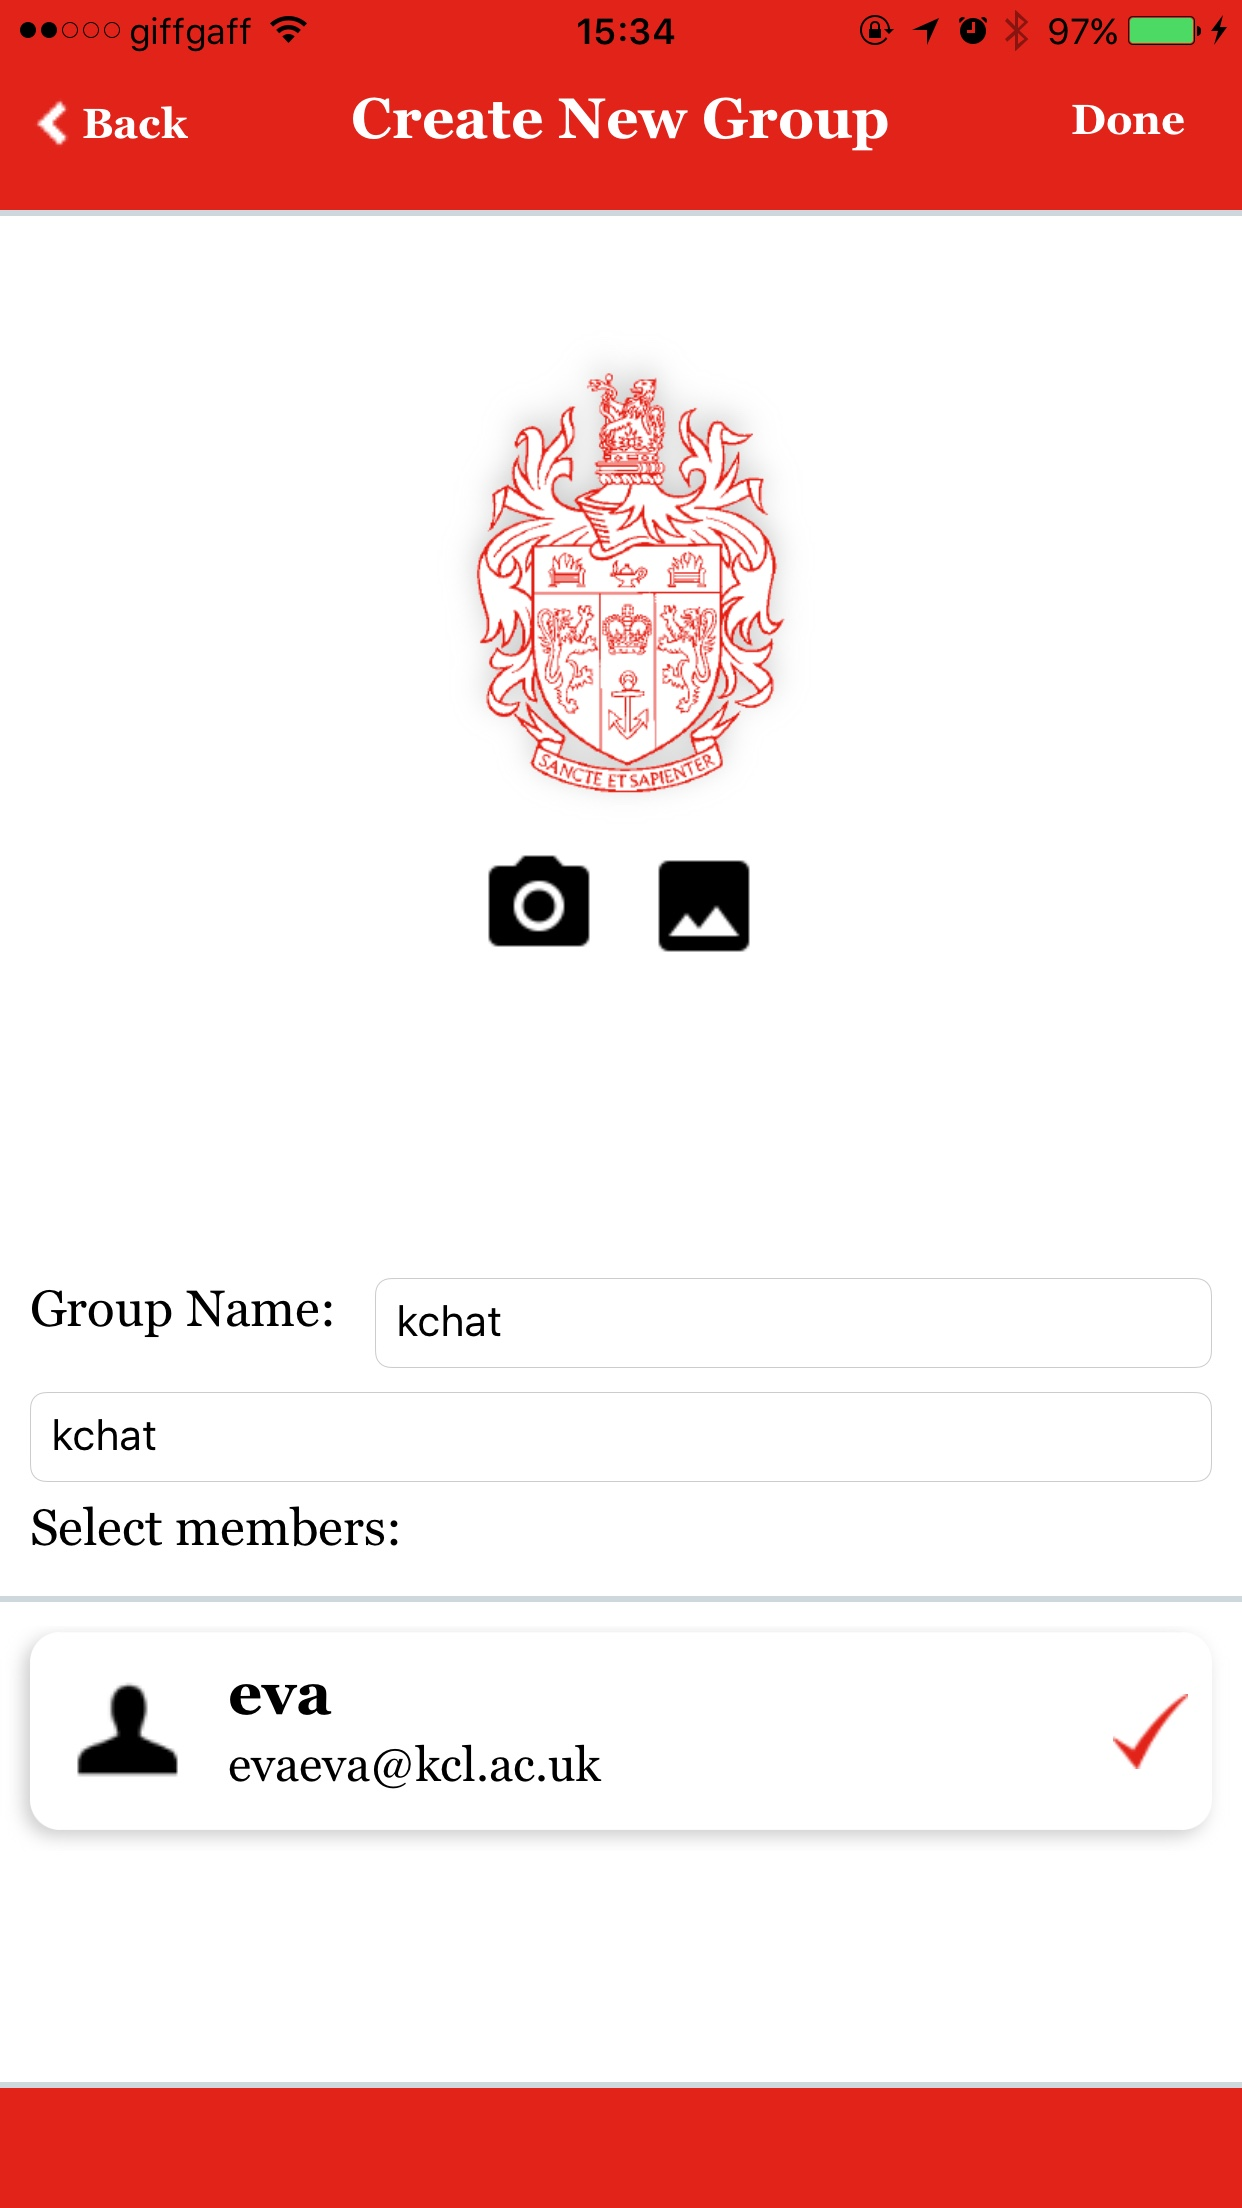
\includegraphics[width=.3\linewidth]{ios1.jpg}\hfill
		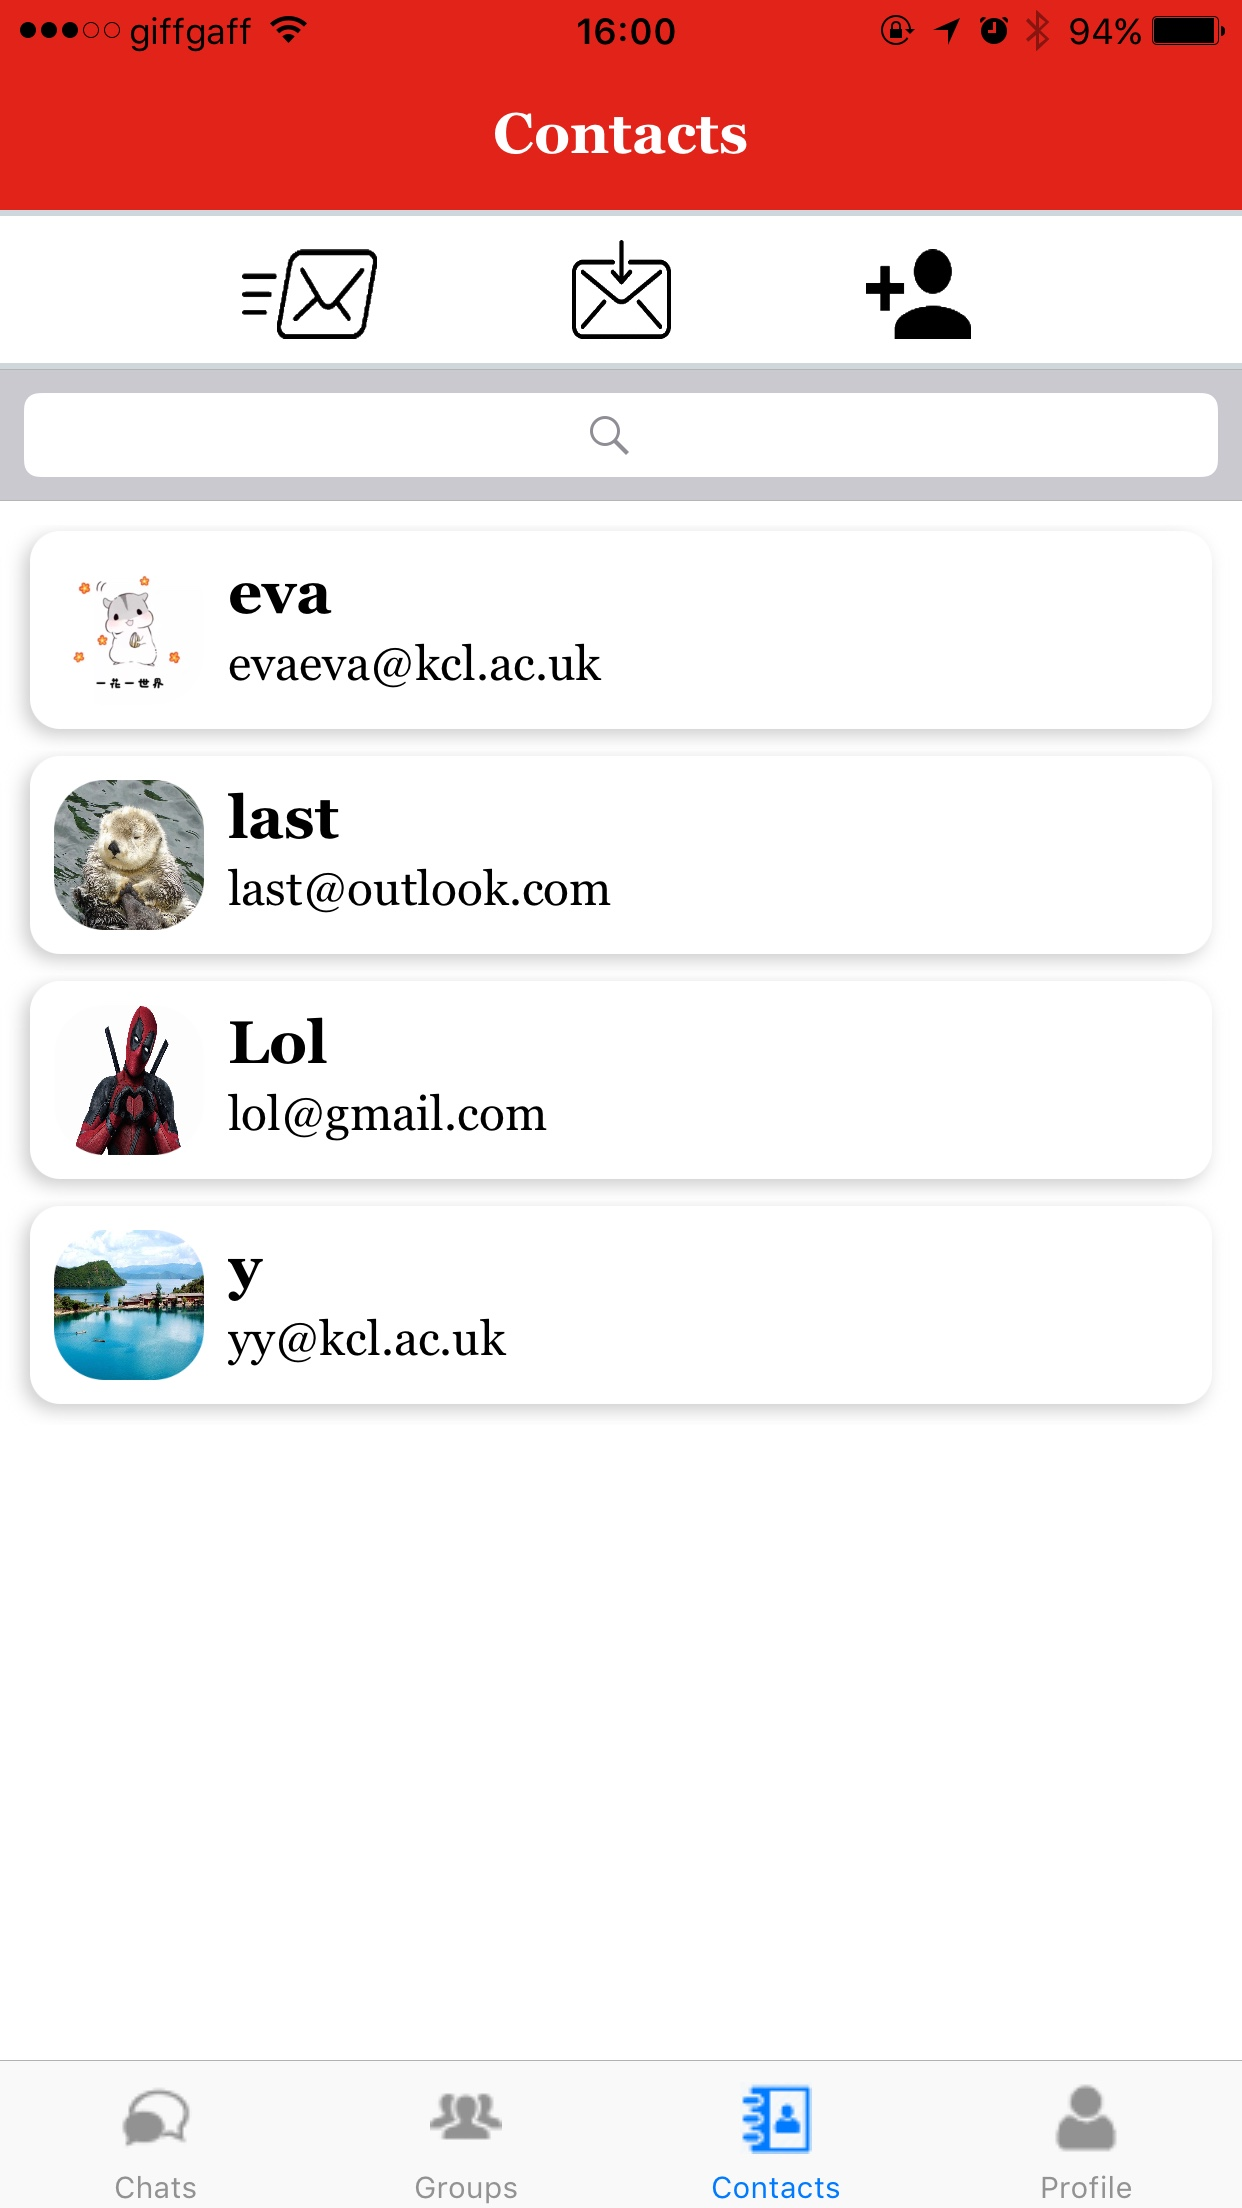
\includegraphics[width=.3\linewidth]{ios2.jpg}\hfill
		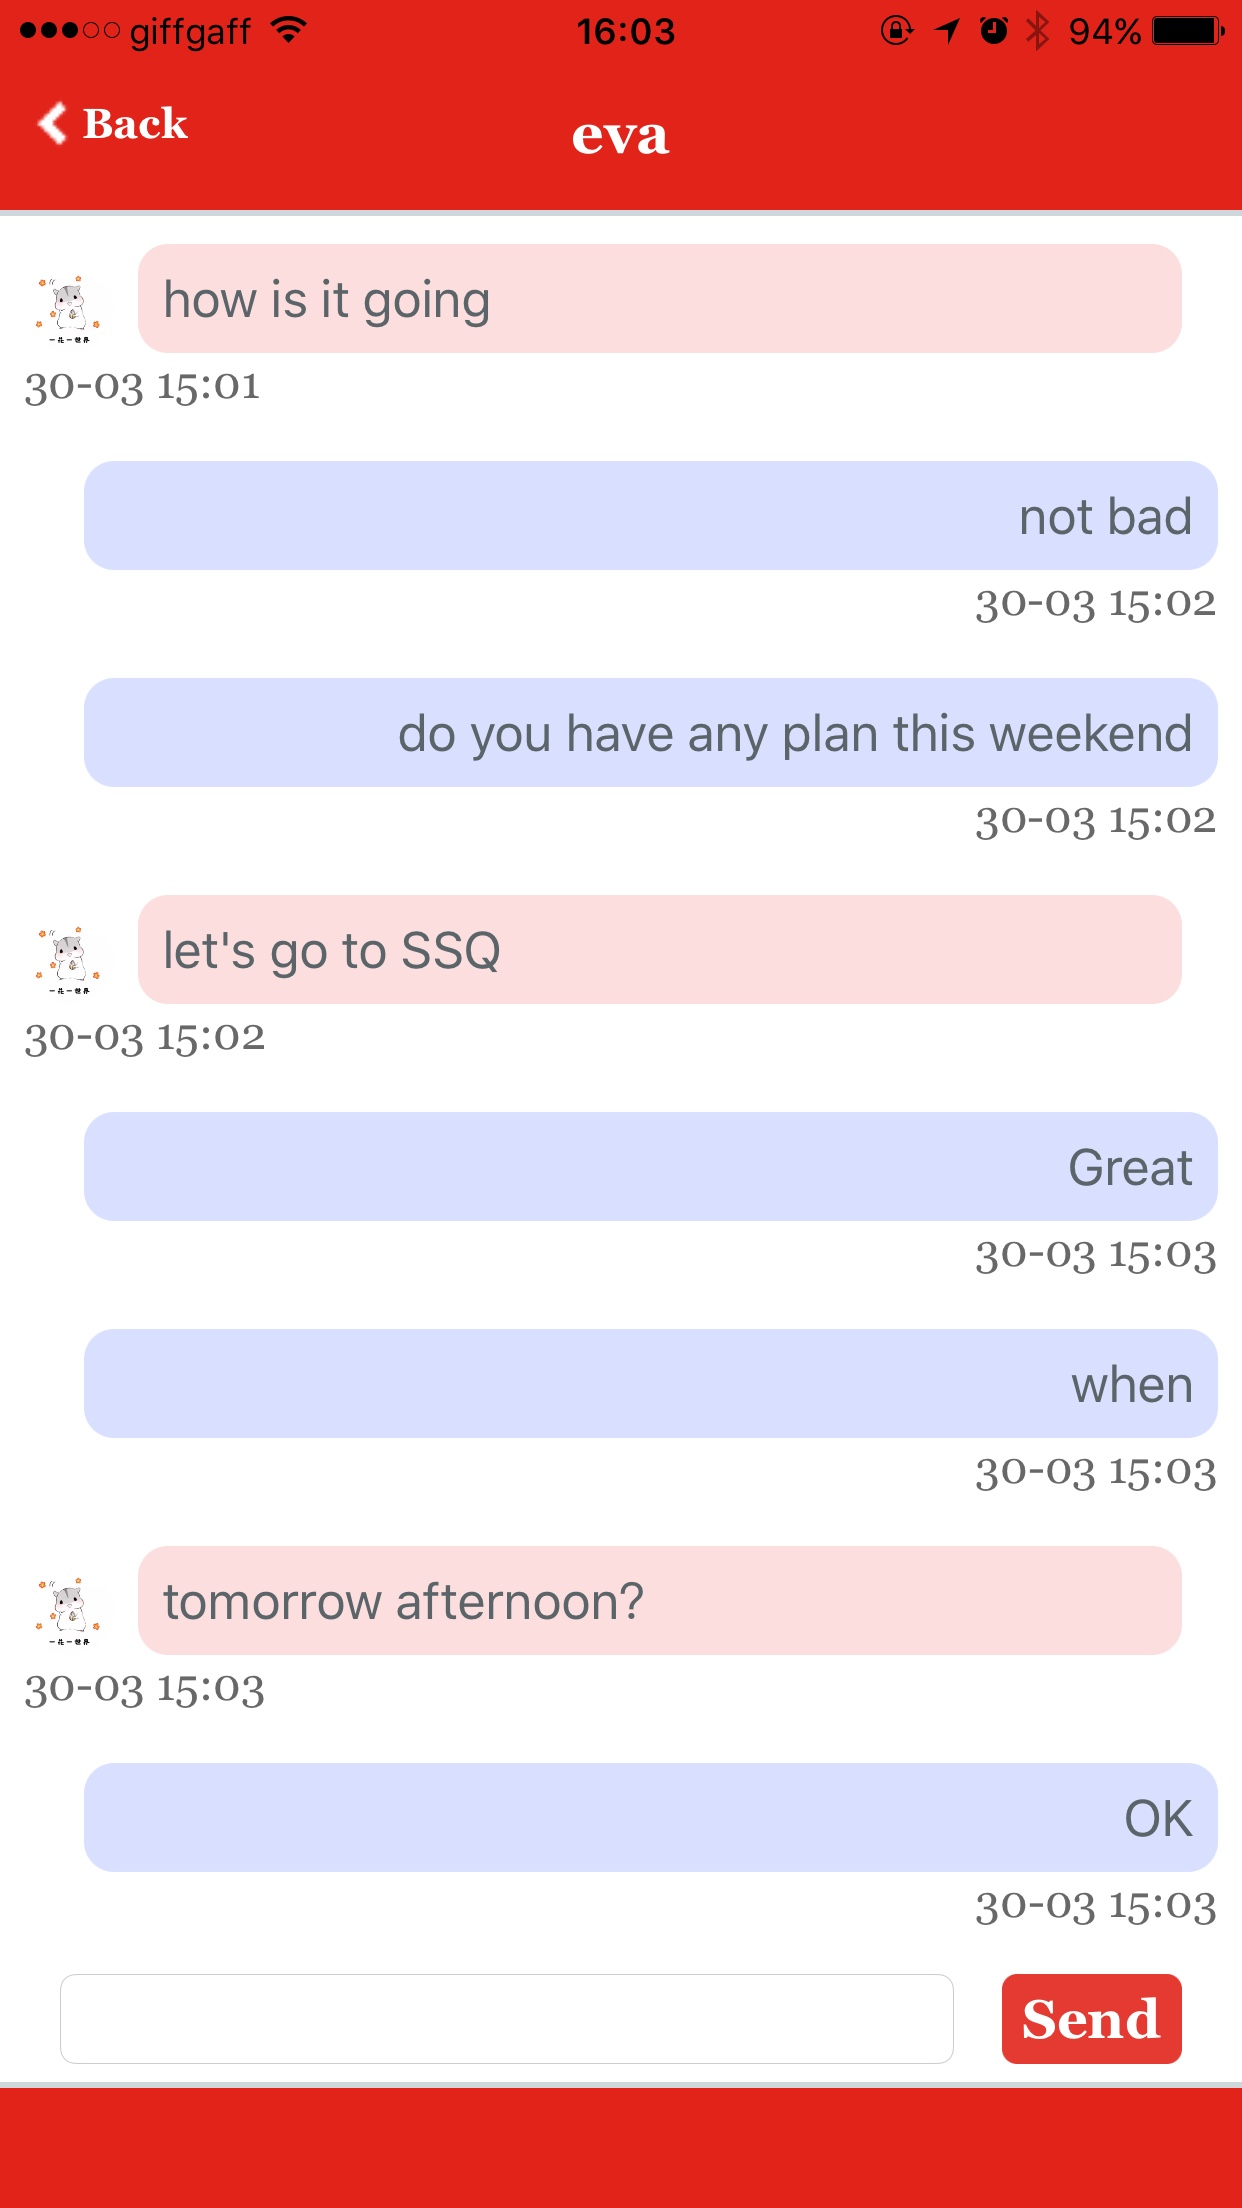
\includegraphics[width=.3\linewidth]{ios3.jpg}
		
	\end{subfigure}\par\medskip
	\caption{Example screen shots of iOS's User Interface}
\end{figure}

\begin{figure}[H]
	\centering
	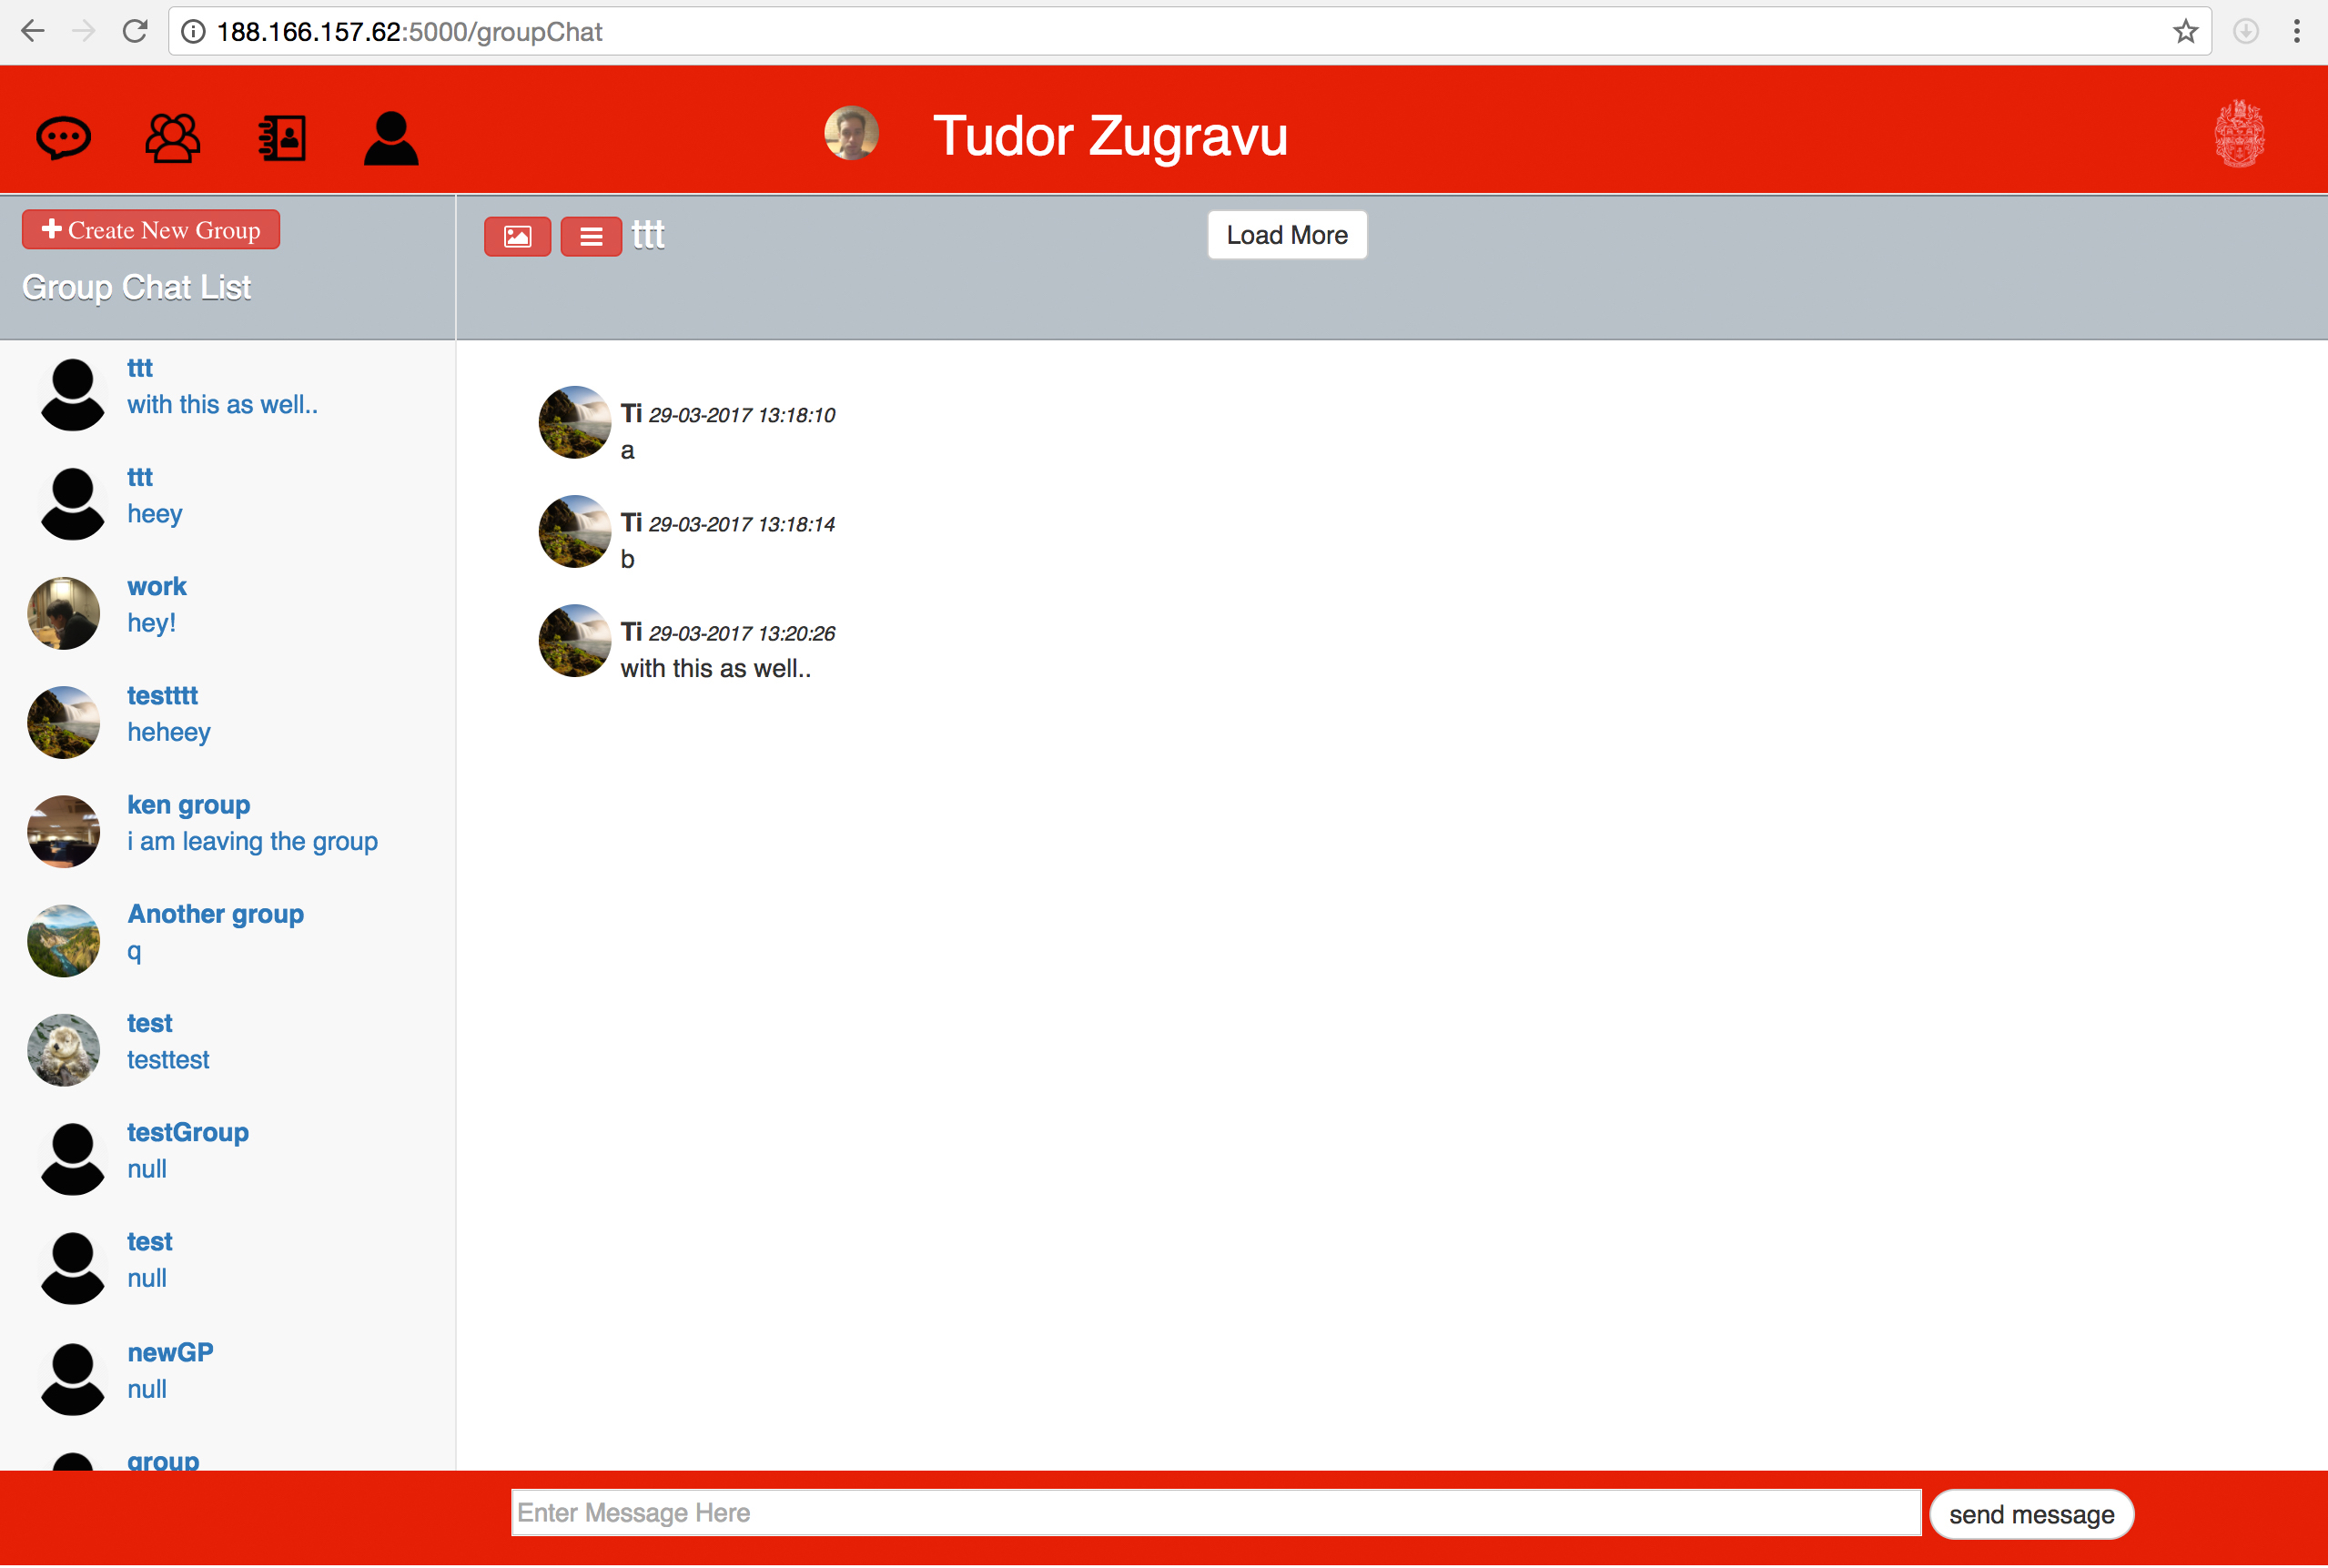
\includegraphics[scale=0.14]{groupChatUI.png}
	\caption{Group Chat UI}
\end{figure}

\begin{figure}[H]
	\centering
	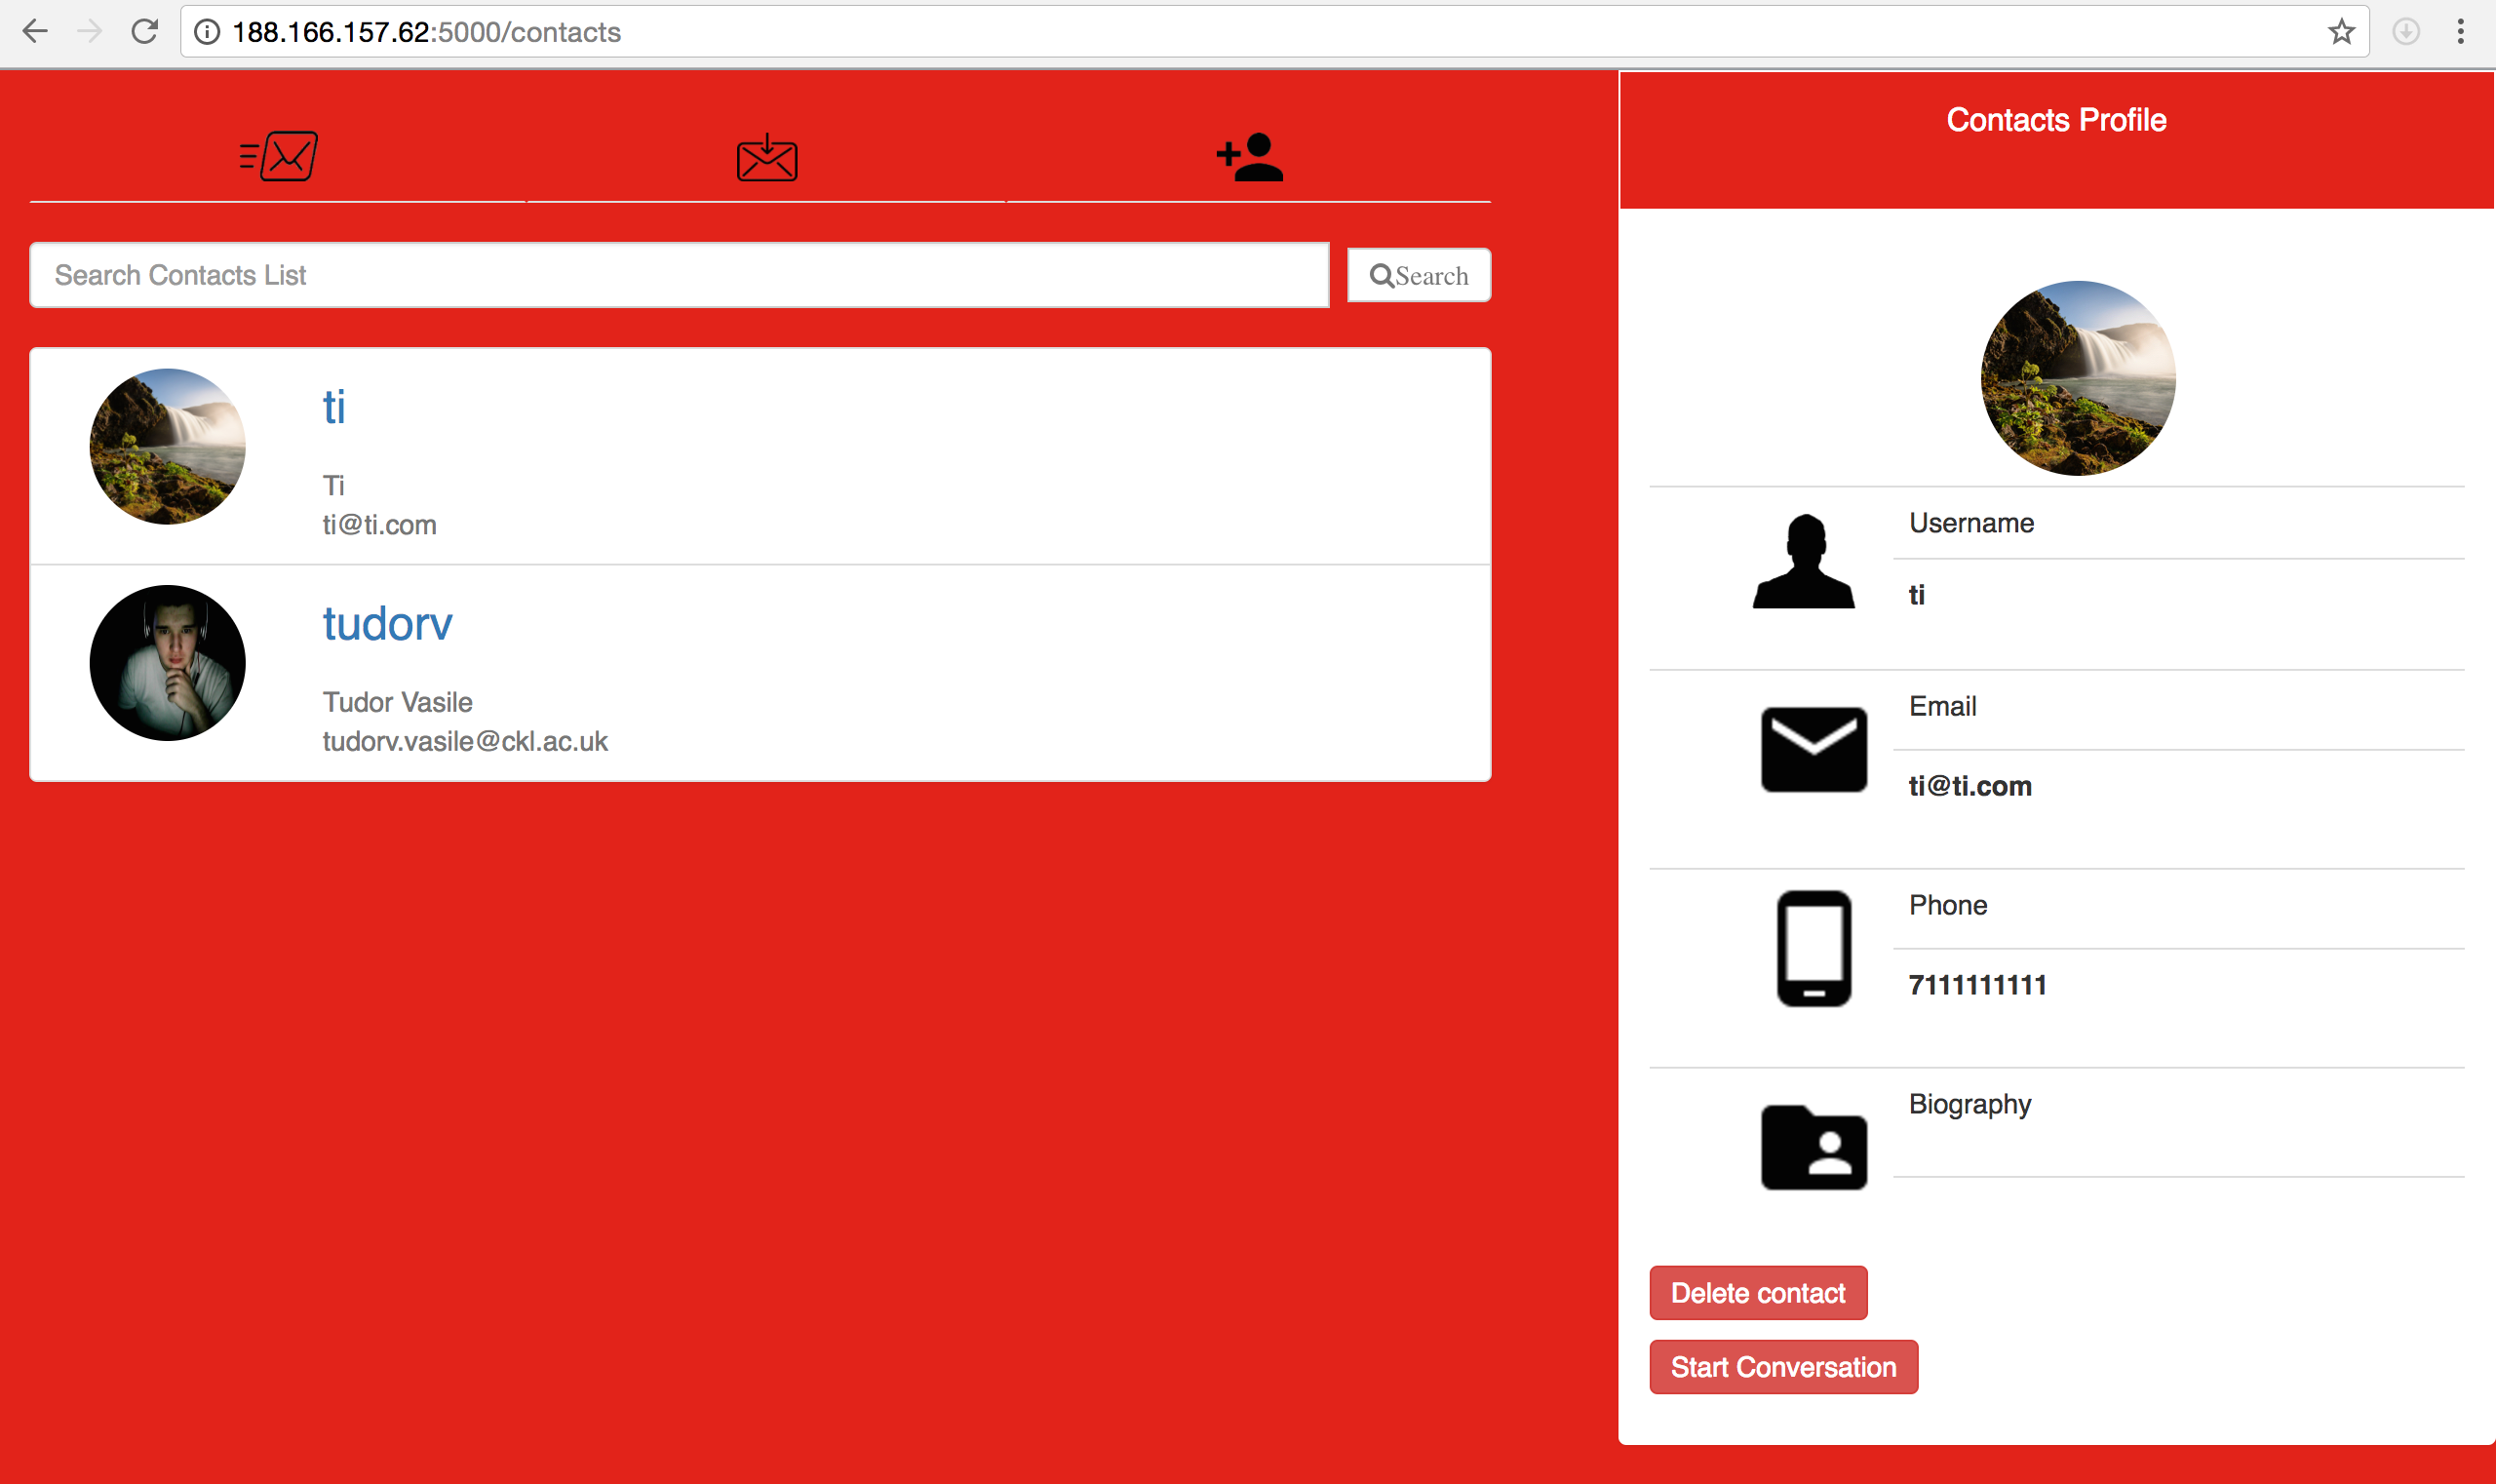
\includegraphics[scale=0.25]{contactsUI.png}
	\caption{Contacts UI}
\end{figure}

\begin{figure}[H]
	\begin{subfigure}{\linewidth}
		\centering
		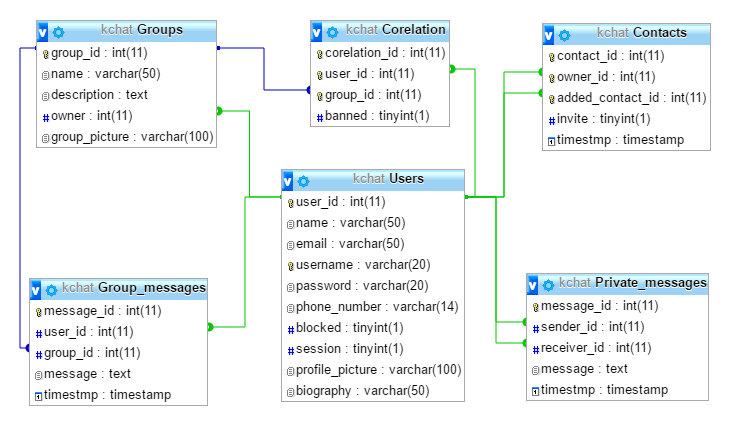
\includegraphics[width=.8\linewidth]{database-straight.png}\hfill
	\end{subfigure}\par\medskip
	\caption{Database design diagram}
\end{figure}

\begin{figure}[H]
	\begin{subfigure}{\linewidth}
		\centering
		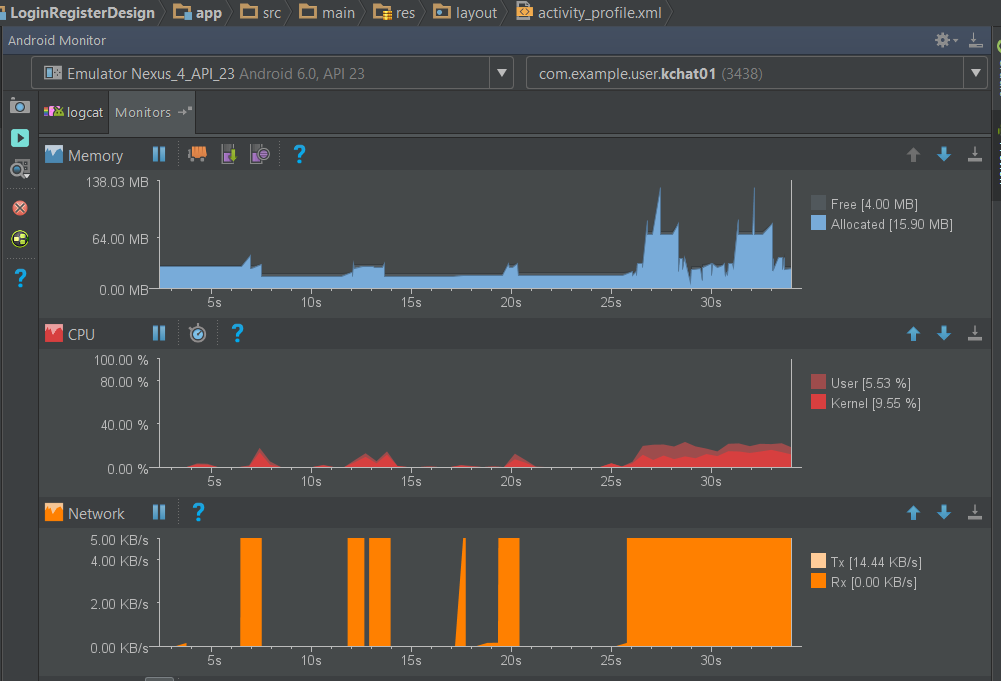
\includegraphics[width=.8\linewidth]{androidtesting.png}\hfill
	\end{subfigure}\par\medskip
	\caption{Database design diagram}
\end{figure}


	\newpage
	 \addcontentsline{toc}{section}{References}
	\begin{thebibliography}{9}
		\bibitem{msnimage} 
		\textit{New version of the popular messaging application  By James Thornton.}. 
		https://msn-messenger.en.softonic.com/

		\bibitem{msndesc} 
		Disadvantages and Advantages of a MSN Messenger in an organisation and as an individual. 
		\textit{Friday, 21 January 2011}. 
		http://lucyakalooose.blogspot.co.uk/2011/01/disadvantages-and-advantages-of-msn.html
		
		\bibitem{facebookmessenger} 
		Messenger
		Sign in with Facebook to get started.
		\textit{}
		https://www.messenger.com/
		
		\bibitem{facebookdesc} 
		Facebook
		From Wikipedia, the free encyclopedia
		\textit{This page was last modified on 23 March 2017, at 21:48}. 
		https://en.wikipedia.org/wiki/Facebook
		
		\bibitem{facebookbattery} 
		How Facebook and Messenger Apps Drain Phone's Battery 
		\textit{Nadeem Unuth
		Updated February 24, 2017}. 
		https://www.lifewire.com/how-facebook-messenger-apps-drains-battery-3880043
		
		\bibitem{imessagedesc} 
		iMessage From Wikipedia, the free encyclopedia 
		\textit{ This page was last modified on 23 March 2017, at 01:20.}. 
		https://en.wikipedia.org/wiki/IMessage
		
		\bibitem{imessagephoto} 
		All-out messaging war between Apple and Facebook heats up
		\textit{Ellis Hamburger  Oct 1, 2012, 1:00pm EDT }. 
		http://www.theverge.com/2012/10/1/3422832/imessage-vs-facebook-messenger
		
		\bibitem{3tierarchitecture} 
		Client/Server Platforms. 
		\textit{by gruppoZenit}. \\
		http://www.gruppozenit.com/ita/software\_applicazioni\_sp\_csa.html
		
			\bibitem{agile}
		Why Should You Use Agile Software Development Methodology?
		\textit{A2 Design Blog}
		http://www.a2design.biz/blog/why-should-you-use-agile-software-development-methodology/
	
	\end{thebibliography}
	
	
	
\end{document}






